\documentclass[11pt]{article}
\usepackage[margin=1in]{geometry}
\usepackage[T1]{fontenc}
\usepackage[utf8]{inputenc}
\usepackage{lmodern}
\usepackage{microtype}
\usepackage{amsmath,amssymb,amsthm,mathtools,bm}
\usepackage{booktabs,array,tabularx,longtable,multirow}
\usepackage{graphicx}
\usepackage[dvipsnames]{xcolor}
\usepackage{enumitem}
\usepackage[backend=biber,style=authoryear,natbib=true,maxcitenames=2,maxbibnames=99,uniquename=false]{biblatex}
\addbibresource{references.bib}
\usepackage{hyperref}
\usepackage[nameinlink,noabbrev]{cleveref}
\usepackage{listings}
\usepackage{caption}
\usepackage{subcaption}
\usepackage{fancyhdr}
\usepackage{setspace}
\usepackage{url}

\definecolor{micblue}{HTML}{174A73}
\definecolor{micgreen}{HTML}{16725D}
\definecolor{micorange}{HTML}{B85C19}
\definecolor{micgray}{HTML}{4C5563}
\hypersetup{
  colorlinks=true,
  linkcolor=micblue,
  citecolor=micgreen,
  urlcolor=micorange,
  pdftitle={Mechanism Interferometry},
  pdfauthor={Jeffrey Emanuel}
}
\pagestyle{fancy}
\fancyhf{}
\lhead{Mechanism Interferometry}
\rhead{Emanuel}
\cfoot{\thepage}
\setlength{\headheight}{14pt}
\setlist{nosep,leftmargin=*}
\onehalfspacing

\newtheorem{theorem}{Theorem}[section]
\newtheorem{proposition}[theorem]{Proposition}
\newtheorem{lemma}[theorem]{Lemma}
\newtheorem{corollary}[theorem]{Corollary}
\newtheorem{definition}[theorem]{Definition}
\newtheorem{assumption}[theorem]{Assumption}
\newtheorem{remark}[theorem]{Remark}
\newtheorem{example}[theorem]{Example}

\newcommand{\E}{\mathbb{E}}
\newcommand{\Pp}{\mathbb{P}}
\newcommand{\Cov}{\operatorname{Cov}}
\newcommand{\Var}{\operatorname{Var}}
\newcommand{\pa}{\operatorname{pa}}
\newcommand{\MB}{\operatorname{MB}}
\newcommand{\OR}{\operatorname{OR}}
\newcommand{\KL}{\operatorname{KL}}
\newcommand{\ess}{\operatorname{ESS}}
\newcommand{\ind}{\mathbbm{1}}
\newcommand{\R}{\mathbb{R}}
\newcommand{\calF}{\mathcal{F}}
\newcommand{\calE}{\mathcal{E}}
\newcommand{\calD}{\mathcal{D}}
\newcommand{\calS}{\mathcal{S}}
\newcommand{\eps}{\varepsilon}
\newcommand{\kAB}{\kappa_{AB}}
\newcommand{\rA}{r_A}
\newcommand{\rB}{r_B}
\newcommand{\rAB}{r_{AB}}
\newcommand{\ellA}{\ell_A}
\newcommand{\ellB}{\ell_B}
\newcommand{\given}{\,\middle|\,}

\title{\textbf{Mechanism Interferometry}\\[0.35em]
\large Auditing the Compositionality of Soft Interventions}
\author{Jeffrey Emanuel\\
\small \href{https://github.com/Dicklesworthstone}{\texttt{@Dicklesworthstone}}}
\date{August 2026}

\begin{document}
\maketitle

\begin{abstract}
We study a system observed under a reference regime, primitive perturbations, and combinations of those perturbations.  For common-support soft interventions, autonomous causal mechanisms impose a rigid algebra on the family of regime distributions.  A primitive intervention that replaces one conditional mechanism has a likelihood ratio local to the target and its parents.  The ratio conditionally normalizes over the target.  Distinct mechanism replacements compose multiplicatively, so mixed finite differences of regime log densities vanish on every square of the factorial design.

These facts yield a finite biconditional certificate on a complete factorial cube.  Relative to a proposed directed acyclic graph and target assignment, locality, targetwise conditional normalization, and zero square curvature on every face are necessary and sufficient for the existence of a context-invariant modular soft-intervention representation.  The certificate extends to a product of finite categorical mechanism families: alternative guides, doses, or implementations within one family may define arbitrary replacement kernels, while every cross-family rectangular log-density contrast must vanish at every background configuration.  The same argument applies to a complete subgrid only when its reference-corner law factorizes over the proposed DAG and its varying-edge ratios are the local normalized primitives.  On an irregular partial design, the null space of the observed main-effects design characterizes all testable flatness restrictions, but flatness alone is not a modularity certificate when the primitive potentials needed to check locality and conditional normalization are unobserved.  A master identity,
\[
\E_0[r_e(X)\mid X_A]=\frac{p_e(X_A)}{p_0(X_A)},
\]
turns orientation into ordinary marginal invariance testing: under a separately justified single-target premise and deletion faithfulness, the target is the coordinate whose deletion leaves the remaining marginal unchanged.  The number of invariant deletions is itself diagnostic: undercoverage can remove edges or create conservative multi-pass abstention, affected descendants generically produce no pass, and balanced parity mechanisms can produce multiple passes.

For two perturbations we define the gauge-invariant mechanism-curvature field
\[
\kappa_{AB}(x)=\log\frac{p_{AB}(x)p_0(x)}{p_A(x)p_B(x)}.
\]
It is the conditional design log-odds ratio after subtracting the known sampling-design odds.  Full-state modularity implies \(\kappa\equiv0\); the converse additionally requires the certificate's locality and conditional-normalization conditions.  Marginalization can create curvature even when the complete mechanisms compose flatly.  We derive the exact identity
\[
e^{\kappa_{AB}(x)}-1=
\frac{\Cov_0(L_A,L_B\mid X=x)}{
\E_0[L_A\mid X=x]\E_0[L_B\mid X=x]},
\]
its Louis missing-information limit, three conservation laws connecting latent conditional coupling to observable ratio-field anticorrelation, and a nested state-expansion identity that turns curvature into a search criterion for missing measurements.

The inferential architecture has two complementary tracks.  With arbitrary regime-conditioned samples and known, state-independent sampling proportions, four-law functionals \(M_w\) identify weighted curvature without an assignment model.  Under product factorial randomization, projected curvature is tested by the Generalised Covariance Measure and its weighted extension, applied to the design bits.  Localization uses the same residual-product machinery; orientation uses simultaneous low-dimensional equivalence tests; flexible multinomial models provide diagnostic interaction fields and compositional prediction.  A running example exhibits maximal outcome synergy with zero complete-state curvature and nonzero outcome-only curvature in closed form.  Simulations cover symmetry-induced orientation failure, latent-state conservation, and implementation inconsistency.  We conclude with protocols for feature-flag experiments, combinatorial Perturb-seq, representation learning, and a memory-safe Rust implementation built on the FrankenPandas, FrankenNumPy, FrankenSciPy, and FrankenTorch ecosystems.
\end{abstract}

\noindent\textbf{Keywords:} causal modularity; soft interventions; density ratios; conditional odds ratios; factorial experiments; mechanism changes; causal representation learning; missing information; conditional independence.

\tableofcontents
\newpage

\section{Introduction}

Empirical interaction is easy to detect and hard to interpret.  A pair of perturbations can look synergistic because the response function is nonlinear, because the perturbations alter one another's mechanisms, because the measured state omits variables that would separate the mechanisms, or because the combined intervention is implemented differently from the two single interventions.  Standard outcome-scale interaction statistics generally mix these possibilities.  A causal analysis needs an object that lives at the level of the complete data-generating law rather than at the level of one selected response summary.

This paper develops such an object from a simple cancellation argument.  Suppose a baseline density factorizes over a directed acyclic graph (DAG), and a soft intervention replaces exactly one conditional mechanism.  In the likelihood ratio between the perturbed and baseline regimes, every unchanged mechanism cancels.  The ratio is therefore supported only on the target and its direct parents.  Because the replacement is a normalized conditional law, the ratio has conditional mean one over the target.  When several distinct replacements are applied together, their ratios multiply.  In log-density space, autonomous mechanism changes add exactly even when observable outcomes interact violently.

The resulting calculus is most transparent when the complete factorial regime family is treated as a single function-valued log-linear model,
\begin{equation}
\log p_s(x)=\log p_0(x)+\sum_{j=1}^K s_j\ell_j(x),
\qquad s\in\{0,1\}^K.
\label{eq:master-loglinear}
\end{equation}
The absence of design-by-design-by-state interactions is equivalent to zero mixed finite differences of \(\log p_s(x)\) on the design cube.  The potentials \(\ell_j\) depend on a reference corner; their mixed differences do not.  This motivates the name \emph{mechanism interferometry}: the experiment is read not only through the displacement of each regime, but through cycle-closure residuals among regimes.

The closest ingredients are classical or already present in neighboring literatures.  Local mechanism shifts underlie causal discovery from changes, uncertain intervention targets, and Joint Causal Inference \citep{tian2001changes,eaton2007interventions,mooij2020jci,squires2020utigsp,brouillard2020dcdi}.  Radon--Nikodym ratios are ordinary change-of-measure objects, recently emphasized as causal density functions \citep{mahadevan2026density}.  The pairwise product law and four-corner contrast have been used directly to discover interactions from unstructured data \citep{xu2024pairwise}.  Conditional odds ratios, collapsibility, missing-information decompositions, and residual-product conditional-independence tests have mature theories \citep{chen2007odds,tchetgen2010odds,greenland1999collapsibility,louis1982missing,shah2020gcm,scheidegger2022wgcm}.  The contribution here is the assembly: these facts are made to constrain one another in an overdetermined certificate and an executable audit protocol.

\subsection{Contributions}

The paper makes eight main contributions.

\begin{enumerate}
\item \textbf{A finite biconditional certificate.}  For a complete factorial family of common-support soft interventions with proposed distinct targets, locality, conditional normalization, and zero curvature on every two-dimensional design face are necessary and sufficient for a modular causal representation.  The result holds for finite categorical mechanism families when every cross-family rectangle is flat at every background; it imposes no linearity among alternative levels of the same family.  On an irregular partial design, the full estimable lack-of-fit contrast space gives the complete flatness audit, while a modularity certificate additionally requires feasible local, normalized primitive potentials.

\item \textbf{Ratio-free orientation.}  Under separately justified single-target intervention semantics and deletion faithfulness, the identity \(\E_0[r_e\mid X_A]=p_e(X_A)/p_0(X_A)\) converts target orientation into low-dimensional two-sample equivalence tests.  It also pins the otherwise unidentified additive constant of an unnormalized discriminative log-ratio score.

\item \textbf{Support-error diagnostics.}  Omitted parents cannot create a unique wrong target but can remove edges or create additional passes; unaffected nondescendants can survive until pruning; and affected descendants generically make every deletion fail.  Zero, one, or multiple invariant deletions become model diagnostics rather than merely estimator outputs, conditional on the separately stated intervention-family assumptions.

\item \textbf{Gauge-invariant curvature and conservation laws.}  We identify curvature with excess conditional design log odds and derive exact balance identities linking weighted curvature, observable ratio covariance, and hidden conditional likelihood-factor covariance.

\item \textbf{A missing-information interpretation.}  Infinitesimal observed curvature is the conditional covariance of complete-state intervention scores, precisely the off-diagonal missing-information term in Louis's decomposition.  A nested covariance identity shows how adding measurements recovers missing mechanism information in stages.

\item \textbf{Two coherent inference tracks.}  Four-law moment functionals apply to regime-conditioned samples with arbitrary known state-independent sampling proportions.  Under product factorial randomization, the GCM and weighted GCM provide orthogonal, cross-fitted tests of projected curvature.  The distinction prevents a subtle but consequential misuse of residual-product tests under arbitrary corner quotas.

\item \textbf{Partial-design geometry.}  On an arbitrary observed binary or categorical design, testable flatness is exactly the lack-of-fit space of a main-effects-only design matrix with a function-valued response.  The causal completion fiber may nevertheless be empty, point identified, or set identified; algebraic testability is a separate axis from causal feasibility.

\item \textbf{An auditable empirical and software protocol.}  We specify localization, orientation, curvature testing, overlap gates, compositional prediction, state expansion, simulations, engineered feature-flag validation, Perturb-seq analysis, and a safe-Rust implementation architecture.  The current release implements the exact algebra, design audits, fail-closed gates, proposal boundaries, and reference diagnostics; the scalable cross-fitted estimator and autonomous mechanism-dictionary loop remain research and implementation targets rather than claimed results.
\end{enumerate}

\section{Setup and scope}

\subsection{Baseline causal model}

Let \(X=(X_1,\ldots,X_d)\) be a complete causal state taking values in a standard measurable space.  Under a baseline regime, assume the density \(p_0\) factorizes over a DAG \(G\):
\begin{equation}
p_0(x)=\prod_{i=1}^d p_i^0(x_i\mid x_{\pa(i)}).
\label{eq:baseline-factorization}
\end{equation}
The reference measure is suppressed.  Equalities involving densities hold almost everywhere on their common support.

There are \(K\) primitive perturbations.  A design corner is \(s=(s_1,\ldots,s_K)\in\{0,1\}^K\), and \(P_s\) denotes the state law under that corner.  The all-zero corner is denoted \(0\).  The primitive corner that activates only perturbation \(j\) is \(e_j\).

\begin{assumption}[Common support]
For every regime used in a ratio or cycle contrast, \(P_s\) and \(P_0\) are mutually absolutely continuous on a common support.
\end{assumption}

Define the density ratio and log-density ratio
\begin{equation}
r_s(x)=\frac{p_s(x)}{p_0(x)},
\qquad
\ell_s(x)=\log r_s(x).
\end{equation}
Common support is not cosmetic.  Under \(P_0\),
\begin{equation}
\Var_0(r_s)=\E_0[r_s^2]-1=\chi^2(P_s\Vert P_0),
\end{equation}
so power and estimator stability deteriorate directly with overlap.  Deterministic hard interventions on continuously distributed variables are often singular; the present theory is therefore a soft-intervention calculus.  Infinitesimal score fields are the natural limit object when perturbations become small.

\subsection{Modular soft interventions}

\begin{definition}[Primitive modular replacement]
Primitive perturbation \(j\) targets node \(t_j\) if it replaces the baseline conditional mechanism \(p_{t_j}^0\) by a valid conditional density \(q_j\), while all other conditional mechanisms remain unchanged:
\begin{equation}
p_{e_j}(x)=q_j(x_{t_j}\mid x_{\pa(t_j)})
\prod_{i\ne t_j}p_i^0(x_i\mid x_{\pa(i)}).
\end{equation}
\end{definition}

\begin{definition}[Context-invariant composition]
Primitive replacements compose context-invariantly if, whenever perturbation \(j\) is active in a combination, it uses the same \(q_j\) that it uses alone.  For distinct targets,
\begin{equation}
p_s(x)=
\prod_{j:s_j=1}q_j(x_{t_j}\mid x_{\pa(t_j)})
\prod_{i\notin\{t_j:s_j=1\}}p_i^0(x_i\mid x_{\pa(i)}).
\label{eq:modular-combination}
\end{equation}
\end{definition}

Consistent composition is the most load-bearing empirical assumption in the paper.  In combinatorial gene perturbation, guide competition, position effects, and dosage changes can make a nominal perturbation different in a pair than alone.  In software systems, two feature flags can compete for a shared queue, memory budget, or rate limit.  Such effects are scientifically important, but they are implementation curvature rather than evidence that an otherwise correctly implemented complete causal state is insufficient.

\section{Locality, normalization, and the augmented regime graph}

\subsection{A global perturbation has a local ratio}

For a primitive replacement at \(t\), all unchanged factors cancel:
\begin{equation}
r_e(x)=\frac{p_e(x)}{p_0(x)}
=\frac{q_e(x_t\mid x_{\pa(t)})}{p_t^0(x_t\mid x_{\pa(t)})}.
\label{eq:local-ratio}
\end{equation}
Thus \(r_e\) is measurable with respect to
\begin{equation}
F_t=\{t\}\cup\pa(t).
\end{equation}
Descendants can move dramatically in marginal distribution, but their downstream mechanisms cancel in the joint ratio.

Let \(E\) be a binary label distinguishing regime \(e\) from baseline, with pooled sampling probabilities \(\rho_e,\rho_0\).  Bayes' rule gives
\begin{equation}
\log\frac{\Pp(E=e\mid X=x)}{\Pp(E=0\mid X=x)}
=
\log\frac{\rho_e}{\rho_0}+\ell_e(x).
\label{eq:classifier-ratio}
\end{equation}
Therefore
\begin{equation}
E\perp X_{-F_t}\mid X_{F_t}.
\label{eq:regime-mb}
\end{equation}
In the augmented DAG with context edge \(E\to X_t\), \(F_t\) is the Markov blanket of \(E\): its child and the child's other parents.  Localization is therefore not an escape from conditional-independence testing.  It relocates the search from state--state relations to design--state relations, where the target variable is discrete, externally assigned in experiments, and low-dimensional.

\subsection{Conditional normalization orients the family}

Because \(q_e(\cdot\mid x_{\pa(t)})\) is a conditional density,
\begin{equation}
\E_0[r_e(X)\mid X_{\pa(t)}]=1.
\label{eq:conditional-normalization}
\end{equation}
This asymmetry distinguishes the child from its parents.  The same condition will later be turned into a ratio-free marginal test.

\section{The gauge field on the intervention cube}

\subsection{Mixed finite differences}

Let
\begin{equation}
h_s(x)=\log p_s(x).
\end{equation}
For a set \(T\subseteq[K]\) and a base corner \(b\) with \(b_j=0\) for every \(j\in T\), define
\begin{equation}
\kappa_T^b(x)
=
\Delta_T h(b;x)
=
\sum_{U\subseteq T}(-1)^{|T|-|U|}h_{b+\mathbf{1}_U}(x).
\label{eq:mobius-curvature}
\end{equation}
For two perturbations \(A,B\) at the reference corner,
\begin{equation}
\boxed{
\kappa_{AB}(x)=
\log\frac{p_{AB}(x)p_0(x)}{p_A(x)p_B(x)}.
}
\label{eq:pair-curvature}
\end{equation}
Equivalently,
\begin{equation}
r_{AB}(x)=r_A(x)r_B(x)e^{\kappa_{AB}(x)}.
\label{eq:curvature-factor}
\end{equation}

\subsection{Gauge invariance}

Adding any field of the form
\begin{equation}
a(x)+\sum_j s_jb_j(x)
\end{equation}
to \(h_s(x)\) leaves every mixed difference of order at least two unchanged.  The primitive potentials are reference-dependent, while the curvature is not.  Reversing a coordinate orientation changes the sign of any mixed difference containing that coordinate, but the flatness statement \(\kappa_T=0\) is invariant.  No scientifically privileged baseline is required.

The analogy with a gauge field is exact at the algebraic level: edge increments are potentials, cycle sums are field strengths, and zero cycle sums are discrete integrability conditions.  In free-energy perturbation, analogous cycle-closure residuals diagnose inconsistency among estimated log free-energy differences, and joint multistate estimators pool evidence across states \citep{shirts2008mbar}.  Here the response is not a scalar free energy but the full function \(x\mapsto\log p_s(x)\).

\subsection{Conditional design odds}

Let \(A,B\in\{0,1\}\) be the design bits, and let \(\rho_{ab}\) be the state-independent probabilities with which observations from the four regime laws are pooled.  Write
\begin{equation}
q_{ab}(x)=\Pp_\rho(A=a,B=b\mid X=x).
\end{equation}
Bayes' rule yields
\begin{equation}
\boxed{
\kappa_{AB}(x)=
\log\frac{q_{11}(x)q_{00}(x)}{q_{10}(x)q_{01}(x)}
-
\log\frac{\rho_{11}\rho_{00}}{\rho_{10}\rho_{01}}.
}
\label{eq:sampling-odds-anchor}
\end{equation}
Thus curvature is excess conditional design log odds after subtracting the known pooled-design odds.  The density functional includes its constant component.  A free-intercept multinomial parametrization can hide that component only if the analyst reports a centered interaction term rather than reconstructing the complete posterior odds and subtracting \(\log\OR(\rho)\).

Equation \eqref{eq:sampling-odds-anchor} survives arbitrary known state-independent corner quotas.  It fails under within-regime state-dependent selection: if inclusion depends on \(X\) given the regime, the sampled conditional law is not \(p_s\), and the four-law density curvature is no longer recovered without modeling selection.

\section{The finite certificate}

\begin{theorem}[Finite modular soft-intervention certificate]
\label{thm:certificate}
Assume that the complete factorial family \(\{p_s:s\in\{0,1\}^K\}\) is observed, \(p_0\) factorizes over a proposed DAG \(G\), all regimes have common support, and primitive perturbations are assigned distinct proposed targets \(t_1,\ldots,t_K\).  Let
\begin{equation}
r_j(x)=\frac{p_{e_j}(x)}{p_0(x)}.
\end{equation}
The following are equivalent.

\begin{enumerate}[label=(\Alph*)]
\item There exist valid conditional mechanisms \(q_j(x_{t_j}\mid x_{\pa(t_j)})\) such that perturbation \(j\) replaces only mechanism \(t_j\), the replacement is context-invariant, and the resulting modular factorization reproduces every \(p_s\).

\item The following three conditions hold:
\begin{enumerate}[label=(\roman*)]
\item \emph{Locality:}
\begin{equation}
r_j(x)=r_j(x_{t_j},x_{\pa(t_j)}).
\end{equation}
\item \emph{Conditional normalization:}
\begin{equation}
\E_0[r_j(X)\mid X_{\pa(t_j)}]=1.
\end{equation}
\item \emph{Square flatness:} for every pair \(j\ne k\) and every base corner \(b\) on which the corresponding two-dimensional face is defined,
\begin{equation}
\kappa_{jk}^b(x)=0.
\end{equation}
\end{enumerate}
\end{enumerate}
\end{theorem}

\begin{proof}
If (A) holds, factor cancellation gives locality, integration of each replacement conditional gives normalization, and context-invariant composition gives
\begin{equation}
\frac{p_s(x)}{p_0(x)}=\prod_j r_j(x)^{s_j}.
\end{equation}
Every mixed finite difference of order at least two therefore vanishes.

Conversely, define
\begin{equation}
q_j(x_{t_j}\mid x_{\pa(t_j)})
=
r_j(x_{t_j},x_{\pa(t_j)})p_{t_j}^0(x_{t_j}\mid x_{\pa(t_j)}).
\label{eq:constructed-kernel}
\end{equation}
Locality gives the correct arguments and normalization makes \(q_j\) a valid conditional density.  It remains to show that square flatness implies global multiplicative composition.  For \(s_j=0\), set
\begin{equation}
\delta_j(s;x)=h_{s+e_j}(x)-h_s(x).
\end{equation}
Zero \((j,k)\)-face curvature gives
\begin{equation}
\delta_j(s+e_k;x)=\delta_j(s;x).
\end{equation}
The \((K-1)\)-cube with coordinate \(j\) fixed is connected, so \(\delta_j(s;x)\) is independent of every other design coordinate.  Hence it equals its value at the reference corner, \(\ell_j(x)\).  Summing edge increments along any path from \(0\) to \(s\),
\begin{equation}
h_s(x)=h_0(x)+\sum_j s_j\ell_j(x).
\end{equation}
Therefore \(p_s=p_0\prod_jr_j^{s_j}\), which is exactly the density generated by replacing the baseline kernels with \eqref{eq:constructed-kernel}.  This proves (A).
\end{proof}

\begin{theorem}[Categorical mechanism-family certificate]
\label{thm:categorical-certificate}
For each mechanism family \(j\), let \(\mathcal A_j\) be a finite level set
with marked baseline level \(0_j\), and observe the complete product grid
\(\mathcal S=\prod_{j=1}^K\mathcal A_j\).  Nonbaseline levels of one family are
mutually exclusive alternative replacements of the same proposed target
\(t_j\); targets remain distinct across families.  Assume common support and
that \(p_0\) factorizes over the proposed DAG.  For \(a\ne0_j\), let
\begin{equation}
r_{j,a}(x)=\frac{p_{(0_1,\ldots,a,\ldots,0_K)}(x)}{p_0(x)}.
\end{equation}
The grid admits a context-invariant modular representation by valid
family-level replacement kernels if and only if:
\begin{enumerate}[label=(\roman*)]
\item \(r_{j,a}\) is measurable with respect to
\(X_{t_j},X_{\pa(t_j)}\) for every \(j,a\);
\item
\begin{equation}
\E_0[r_{j,a}(X)\mid X_{\pa(t_j)}]=1
\end{equation}
for every \(j,a\); and
\item for every \(j\ne k\), levels \(a,a'\in\mathcal A_j\),
\(b,b'\in\mathcal A_k\), and background
\(u\in\prod_{\ell\notin\{j,k\}}\mathcal A_\ell\),
\begin{equation}
h_{a,b,u}+h_{a',b',u}-h_{a,b',u}-h_{a',b,u}=0
\quad\text{a.e.}
\label{eq:categorical-rectangle}
\end{equation}
It is equivalent in (iii) to take \(a'=0_j,b'=0_k\), but those
baseline-level rectangles must still be checked at every background \(u\).
\end{enumerate}
\end{theorem}

\begin{proof}
Under a modular representation, unchanged DAG factors cancel and the active
family-level kernel ratios multiply, proving all three conditions.  Conversely,
define the increment from family baseline to level \(a\) at background
\(s_{-j}\) by
\begin{equation}
\delta_{j,a}(s_{-j};x)=h_{a,s_{-j}}(x)-h_{0_j,s_{-j}}(x).
\end{equation}
Equation~\eqref{eq:categorical-rectangle}, with the other family's baseline as
one side of the rectangle, makes this increment invariant to changing any
other coordinate to any of its levels.  Hence
\(\delta_{j,a}=\log r_{j,a}\).  Summing increments along a path through the
product grid gives
\begin{equation}
h_s=h_0+\sum_{j:s_j\ne0_j}\log r_{j,s_j}.
\end{equation}
Locality supplies the arguments of each replacement kernel and conditional
normalization makes
\(q_{j,a}=p^0_{t_j}r_{j,a}\) a valid conditional law.  Their modular product
therefore reproduces every \(p_s\).
\end{proof}

The theorem asserts no linear or ordered relation among levels within a
family.  A weak dose and a strong dose may be unrelated normalized replacement
kernels; a continuous dosage path requires its own parameter-dependent
normalization model.  Checking only rectangles whose other coordinates are all
at baseline is also insufficient when \(K\ge3\): a family with
\(h_s=h_0\) at every corner except a normalized nontrivial ratio at \(111\)
passes all such baseline-background faces while failing the opposite faces.

\begin{corollary}[Order two suffices]
On a complete Boolean cube or complete subcube, zero curvature on every square implies that every higher-order M\"obius coefficient vanishes.
\end{corollary}

The theorem is an existence result.  It says that a proposed graph and target assignment admit a modular causal realization of the observed regime family.  Faithfulness and intervention coverage are required to infer that proposal uniquely from data.

\section{The master marginal identity and target orientation}

\begin{lemma}[Master marginal identity]
\label{lem:master-marginal}
For every regime \(e\) and coordinate subset \(A\),
\begin{equation}
\boxed{
\E_0[r_e(X)\mid X_A]
=
\frac{p_e(X_A)}{p_0(X_A)}.
}
\label{eq:master-marginal}
\end{equation}
\end{lemma}

\begin{proof}
For every bounded measurable \(g(X_A)\),
\begin{equation}
\E_0[g(X_A)r_e(X)]=\E_e[g(X_A)]
=\E_0\left[g(X_A)\frac{p_e(X_A)}{p_0(X_A)}\right].
\end{equation}
Uniqueness of conditional expectation proves the result.
\end{proof}

The unconditional special case is \(\E_0[r_e]=1\).  If a discriminative model learns an unnormalized score \(g_e(x)=\ell_e(x)+c\), the constant can be pinned on held-out baseline data by
\begin{equation}
\widehat\ell_e(x)=g_e(x)-\log\widehat\E_0[e^{g_e(X)}].
\label{eq:score-normalization}
\end{equation}

More importantly, the orientation condition becomes a plain marginal invariance statement.  Let \(S\) be a candidate support containing the target \(t\).  For every \(v\in S\), define the deletion hypothesis
\begin{equation}
H_v:\quad P_e^{X_{S\setminus\{v\}}}=P_0^{X_{S\setminus\{v\}}}.
\label{eq:deletion-null}
\end{equation}
By \cref{lem:master-marginal}, this is equivalent to
\begin{equation}
\E_0[r_e(X)\mid X_{S\setminus\{v\}}]=1.
\end{equation}
If \(S=\{t\}\cup S_P\) with \(S_P\subseteq\pa(t)\), deleting \(t\) leaves only pre-intervention nondescendants, so \(H_t\) holds.  Deleting a parent leaves the perturbed target in the tested marginal and generally fails.

\begin{assumption}[Deletion faithfulness]
For the chosen collection of mechanism tilts, the target is the unique coordinate in the localized support whose deletion leaves an invariant marginal.
\end{assumption}

Under deletion faithfulness,
\begin{equation}
\boxed{
t=\text{the unique }v\in S\text{ such that }P_e^{X_{S\setminus\{v\}}}=P_0^{X_{S\setminus\{v\}}}.
}
\end{equation}
This should be estimated by low-dimensional two-sample equivalence tests, not by conditional means of an estimated density ratio.  A global calibration error in \(\widehat r_e\) moves every estimated conditional mean away from one; direct marginal comparison avoids that failure.

\section{Support errors, pass counts, and graph recovery}

Let
\begin{equation}
\operatorname{Pass}(\widehat S)
=
\left\{v\in\widehat S:
P_e^{X_{\widehat S\setminus\{v\}}}=P_0^{X_{\widehat S\setminus\{v\}}}
\right\}.
\end{equation}
Assume initially that \(t\in\widehat S\).

\subsection{Undercoverage}

If
\begin{equation}
\widehat S\subseteq\{t\}\cup\pa(t),
\end{equation}
but the intervention ratio happens not to depend detectably on one or more true parents, then deleting \(t\) still leaves a subset of parents, so the target passes.  Deletion faithfulness on the full family need not survive restriction to \(\widehat S\): omitting a parent can balance a remaining shifted marginal and create an additional pass.  If deletion faithfulness is separately re-established on \(\widehat S\), the target remains unique and the recovered parent set is \(\widehat S\setminus\{t\}\subseteq\pa(t)\).  Without that extra premise, undercoverage can miss edges or force conservative multiple-pass abstention, but it cannot create a unique wrong orientation because the true target still passes.

\subsection{Overcoverage by unaffected nondescendants}

If \(\widehat S\) includes an unaffected nondescendant \(Z\), deleting \(t\) still leaves only variables whose joint marginal is invariant.  The target can remain the unique passing coordinate.  Orientation is robust, but the unpruned candidate parent set can falsely retain \(Z\).  Minimal Markov-boundary localization or a backward pruning stage is still required for exact graph recovery.

\subsection{Affected descendants}

If \(\widehat S\) contains a descendant \(D\) whose marginal law changes, deleting the target leaves \(D\), so the target fails.  Deleting any other coordinate also leaves \(D\).  Deleting \(D\) usually leaves the shifted target family.  Consequently, descendant contamination generically produces no passes.  ``Generically'' is essential: with partial family coverage, deleting the contaminant can leave a specially balanced parity-invariant submarginal.

\subsection{Pass-count audit}

The intended interpretation is therefore
\begin{center}
\begin{tabular}{p{0.18\linewidth}p{0.72\linewidth}}
\toprule
Pass count & Interpretation \\
\midrule
Exactly one & Consistent with unique orientation only after a single-target/locality premise and deletion faithfulness have been established separately. \\
Zero & Descendant contamination, multi-target primitive, selection, implementation mismatch, or insufficient support. \\
More than one & Symmetry, redundancy, deletion-faithfulness failure, or an insufficiently rich set of tilts. \\
\bottomrule
\end{tabular}
\end{center}

The qualification in the one-pass row is essential: pass count cannot validate the single-target premise from the same marginals.  For example, let the baseline on the DAG \(X\to Y\) have independent fair binary variables.  In one perturbed regime, change the root mechanism to \(P_e(X=1)=3/4\) and also change the child mechanism to \(P_e(Y=1\mid X=1)=2/5\), \(P_e(Y=1\mid X=0)=4/5\).  Then \(P_e(Y=1)=1/2\) remains invariant while \(X\) shifts.  Deleting \(X\) is the unique pass on \(\{X,Y\}\), even though both mechanisms changed.  A unique pass orients a family only conditional on independently credible intervention semantics; it does not establish those semantics.

\subsection{A nonpathological parity failure}\label{sec:parity-placeholder}

Let \(P\sim\mathrm{Bernoulli}(1/2)\), \(N\sim\mathrm{Bernoulli}(\eps)\), and define the baseline child
\begin{equation}
T=P\oplus N.
\end{equation}
Under intervention, replace the mechanism by
\begin{equation}
T=\neg P\oplus N.
\end{equation}
The ratio depends on \((P,T)\), but both one-dimensional marginals remain balanced.  Deleting \(T\) leaves the invariant parent marginal; deleting \(P\) leaves the invariant child marginal.  Both coordinates pass.  Balanced parity mechanisms are a live discrete failure mode, not a measure-zero analytic curiosity.

Multiple asymmetric tilts of the same target are the natural remedy.  The target must pass every valid tilt; a spurious symmetry usually does not.  When the experimental record identifies which tilts replace the same target mechanism, taking the union of their localized supports can also reveal parents omitted by a particular intervention.  That grouping is design metadata, not something an unlabeled family multiset generally identifies on its own.

\subsection{Active tilt selection}\label{sec:active-tilt}

The pass-count taxonomy is not only a verdict; it prescribes the next experiment.  Suppose a family reaches the multiple-pass state with competing invariant deletions \(v_1,\ldots,v_m\).  Each competitor \(v_i\) corresponds to the hypothesis that \(v_i\) is the target, and each hypothesis predicts, for any candidate tilt \(q\), which deletion marginals would remain invariant under that tilt.  A discriminating tilt is one whose predicted deletion outcomes differ across the surviving hypotheses.  Given a feasible tilt class \(\mathcal{Q}\), select
\begin{equation}
q^\star
=
\arg\max_{q\in\mathcal Q}\;
\min_{i\ne j}\,
D\!\left(P^{(q)}_{i},\,P^{(q)}_{j}\right),
\label{eq:active-tilt}
\end{equation}
where \(P^{(q)}_{i}\) denotes the deletion-marginal pattern predicted under hypothesis \(i\) and \(D\) is the same discrepancy used for equivalence testing.  Maximizing the worst-case separation targets the residual symmetry directly rather than spending samples uniformly.

In the parity example of \cref{sec:parity-placeholder}, the ambiguity is sustained by the symmetry of the replacement: both competing deletion marginals stay balanced.  The admissible next experiment is another tilt of the same target mechanism, not an intervention on a different node.  Care is needed in choosing it: any replacement of the form \(T=\neg P\oplus N'\) with independent noise \(N'\), however biased, leaves \(T\) exactly uniform, so biasing the noise alone cannot break the tie.  An explicitly asymmetric conditional does: take \(q(T=1\mid P=0)=\alpha\) and \(q(T=1\mid P=1)=\beta\) with \(\alpha+\beta\ne1\) and common support, so that \(\Pp(T=1)=(\alpha+\beta)/2\ne1/2\).  The target's own marginal then moves, the parent-deletion marginal changes while the target-deletion marginal remains invariant, and one additional regime separates the two hypotheses.  The same criterion covers the state-expansion loop: when curvature is found and candidate measurements compete to explain it, \cref{eq:nested-state} predicts each candidate's residual field, and the next measurement is the one whose predictions best separate the surviving explanations.  Orientation, like state expansion, thereby becomes a sequential design problem with an explicit objective, rather than a fixed battery that either succeeds or abstains.

The acquisition score in \eqref{eq:active-tilt} has proposal authority only.  It depends on a predictive model for experiments not yet run, so model misspecification can make the ranking poor even when the eventual certificate remains valid.  Before collecting follow-up data, freeze the surviving hypotheses, feasible tilt library, predicted pairwise separations, model and data fingerprints, random seed, and deterministic tie rule; the software artifact binds the complete ordered candidate library with a derived content fingerprint.  Reject candidates that change a different primitive, lack measurable delivery or common support, or would invoke product-factorial inference without verified product odds or an explicit reweighting plan.  The selected tilt is then a new independently randomized regime and re-enters the audit at preflight; neither its predicted separation nor its rank resolves the original multiple-pass state.  If no candidate survives these feasibility gates, the correct output is an explicit experiment-design abstention rather than a forced target.

\subsection{Recovering the DAG from family sets}
\label{sec:graph-recovery}

If each node receives a sufficiently rich single-target perturbation, orientation gives every family \(\{i\}\cup\pa(i)\) directly.  Even without target labels, the multiset of family sets uniquely determines a DAG.  Process families in topological order.  After removing previously identified nodes, the earliest unidentified node has no unidentified parents, so its reduced family is the singleton containing itself.  Assign it, restore its removed parents, and continue.  A formal proof appears in \cref{app:proofs}.

The one-family-per-node condition is load bearing.  With repeated tilts and no same-target group labels, an undercovered family can peel before a richer family of the same target.  For example, the unlabeled multiset \(\{\{A\},\{B\},\{A,B\}\}\) is compatible with \(A\to B\), one source-family observation for \(A\), and two tilts of \(B\), one of which omits parent \(A\).  The two singleton sets peel simultaneously, after which the remaining set contains no unidentified node and cannot be assigned uniquely.  Thus repeated tilts should be grouped by an independently recorded mechanism/target identifier and unioned before unlabeled peeling; absent that metadata, the reconstruction must abstain rather than infer which already identified member generated the extra family.

\section{Conservation laws}

\subsection{The moment battery}

Exact modularity implies
\begin{equation}
\boxed{
\E_0\left[\prod_{j\in T}r_j(X)\right]=1
\quad\text{for every }T\subseteq[K].
}
\label{eq:moment-battery}
\end{equation}
For a pair,
\begin{equation}
\Cov_0(r_A,r_B)=0.
\end{equation}
The causal families can be statistically dependent; the ratios nevertheless satisfy this orthogonality because their conditional normalizations telescope.

These are inexpensive necessary conditions, but they are not complete.  The exact meaning of the pair statistic follows from \eqref{eq:curvature-factor} and \(\E_0[r_{AB}]=1\):
\begin{equation}
\boxed{
\E_0[r_A r_B]-1
=
-\E_0\left[r_A r_B(e^{\kappa_{AB}}-1)\right].
}
\label{eq:curvature-balance}
\end{equation}
The scalar moment test estimates a signed average of \(e^\kappa-1\) under the ratio-tilted measure proportional to \(r_A r_B\,dP_0\).  Its blind spot is quantitative: sign-varying curvature can integrate to zero.

Suppose \(r_A r_B\in L^1(P_0)\).  For any bounded witness \(w\), define
\begin{equation}
M_w
=
\E_0\left[w(X)\{r_{AB}(X)-r_A(X)r_B(X)\}\right].
\label{eq:Mw}
\end{equation}
Then
\begin{equation}
M_w=
\E_0\left[w(X)r_A(X)r_B(X)(e^{\kappa(X)}-1)\right].
\label{eq:Mw-curvature}
\end{equation}
Under positivity,
\begin{equation}
M_w=0\text{ for every bounded }w
\quad\Longleftrightarrow\quad
\kappa=0\quad P_0\text{-a.s.}
\end{equation}
The scalar battery is the special case \(w\equiv1\).

\subsection{Latent-factor conservation}

Let the complete state be \(Z=(X,U)\), with baseline density \(q_0\).  Suppose \(L_A,L_B\in L^2(P_0)\) and the complete-state regime factors satisfy
\begin{equation}
q_A=q_0L_A,
\qquad
q_B=q_0L_B,
\qquad
q_{AB}=q_0L_AL_B.
\label{eq:latent-flat}
\end{equation}
After marginalizing \(U\),
\begin{equation}
r_A(X)=\E_0[L_A\mid X],
\qquad
r_B(X)=\E_0[L_B\mid X],
\qquad
r_{AB}(X)=\E_0[L_AL_B\mid X].
\label{eq:latent-projections}
\end{equation}
Therefore
\begin{equation}
\boxed{
e^{\kappa_{AB}(x)}-1
=
\frac{\Cov_0(L_A,L_B\mid X=x)}{r_A(x)r_B(x)}.
}
\label{eq:latent-covariance}
\end{equation}
Because \(q_A,q_B,q_{AB}\) are normalized,
\begin{equation}
\E_0[L_A]=\E_0[L_B]=\E_0[L_AL_B]=1,
\end{equation}
so \(\Cov_0(L_A,L_B)=0\).  The law of total covariance gives
\begin{equation}
\boxed{
\Cov_0(r_A,r_B)
=
-\E_0[\Cov_0(L_A,L_B\mid X)].
}
\label{eq:latent-conservation}
\end{equation}
Combining \eqref{eq:latent-covariance} and \eqref{eq:latent-conservation} yields the three-way conservation law
\begin{equation}
\boxed{
\Cov_0(r_A,r_B)
=
-\E_0[r_A r_B(e^{\kappa}-1)]
=
-\E_0[\Cov_0(L_A,L_B\mid X)].
}
\label{eq:three-way-conservation}
\end{equation}

Whatever conditional coupling marginalization creates between flat latent factors must reappear, with opposite sign on average, as correlation between the observable primitive ratio fields.  At orders three and above, Brillinger's conditioning formula decomposes cumulants through sums over set partitions; the clean two-term split in \eqref{eq:latent-conservation} is special to covariance \citep{brillinger1969cumulants}.

\section{Running example: synergy, flatness, and marginal curvature}

Let \(X_1,X_2\in\{-1,+1\}\) be independent Rademacher variables under baseline, and let
\begin{equation}
Y=X_1X_2+\varepsilon,
\qquad
\varepsilon\sim N(0,\sigma^2).
\label{eq:running-system}
\end{equation}
Perturbation \(A\) tilts the source distribution of \(X_1\):
\begin{equation}
P_A(X_1=x)=\frac{1+ax}{2},
\qquad |a|<1.
\end{equation}
Perturbation \(B\) analogously tilts \(X_2\) by \(b\).

\subsection{Complete state}

The primitive ratios are
\begin{equation}
r_A(X_1)=1+aX_1,
\qquad
r_B(X_2)=1+bX_2.
\end{equation}
The combined ratio is their product, so
\begin{equation}
\kappa_{AB}(X_1,X_2,Y)=0.
\end{equation}
The source mechanisms compose autonomously.

\subsection{Outcome synergy}

Yet
\begin{equation}
\E_0[Y]=\E_A[Y]=\E_B[Y]=0,
\qquad
\E_{AB}[Y]=ab.
\end{equation}
Thus the additive outcome interaction is exactly \(ab\).  Neither perturbation alone changes the mean; together they do.  Outcome interaction is a property of a chosen response and scale, whereas mechanism curvature is a property of the full regime law.  This sharpens the distinction between statistical and mechanistic interaction emphasized in classical interaction theory \citep{vanderweele2014interaction}.

\subsection{Retaining only the outcome}

Under either primitive tilt alone, the product \(X_1X_2\) remains symmetric, so
\begin{equation}
p_A(y)=p_B(y)=p_0(y).
\end{equation}
Under the combined tilt,
\begin{equation}
p_{AB}(y)=
\frac{1+ab}{2}\phi_\sigma(y-1)
+
\frac{1-ab}{2}\phi_\sigma(y+1),
\end{equation}
while
\begin{equation}
p_0(y)=\frac12\phi_\sigma(y-1)+\frac12\phi_\sigma(y+1).
\end{equation}
Using
\begin{equation}
\frac{\phi_\sigma(y-1)-\phi_\sigma(y+1)}
{\phi_\sigma(y-1)+\phi_\sigma(y+1)}
=
\tanh\left(\frac{y}{\sigma^2}\right),
\end{equation}
we obtain
\begin{equation}
\frac{p_{AB}(y)}{p_0(y)}
=
1+ab\tanh\left(\frac{y}{\sigma^2}\right)
\end{equation}
and therefore
\begin{equation}
\boxed{
\kappa_{AB}(y)=
\log\left[1+ab\tanh\left(\frac{y}{\sigma^2}\right)\right].
}
\label{eq:tanh-curvature}
\end{equation}

\begin{figure}[t]
\centering
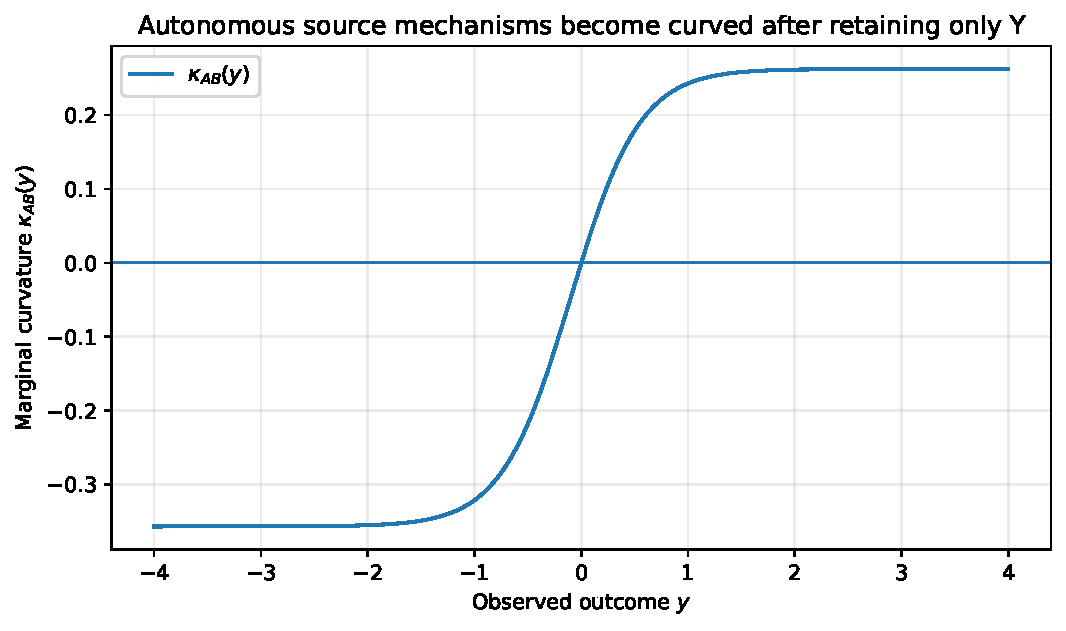
\includegraphics[width=0.84\linewidth]{figures/running_example.pdf}
\caption{For \(a=0.6\), \(b=0.5\), and \(\sigma=0.8\), the complete source mechanisms are flat while the outcome-only representation has sign-varying curvature.}
\label{fig:running-example}
\end{figure}

The example is also the canonical blind spot of the scalar moment battery.  In the \(Y\)-only representation,
\begin{equation}
r_A(y)=r_B(y)=1,
\end{equation}
so \(\E_0[r_A r_B]=1\) passes trivially.  Nevertheless \(\kappa(y)\not\equiv0\).  The weighted mean vanishes because \(p_0\) is symmetric and \(\tanh(y/\sigma^2)\) is odd.

The latent covariance cross-check is immediate:
\begin{equation}
\E_0[X_1\mid Y=y]=\E_0[X_2\mid Y=y]=0,
\end{equation}
while
\begin{equation}
\E_0[X_1X_2\mid Y=y]=\tanh(y/\sigma^2).
\end{equation}
Therefore
\begin{equation}
\Cov_0(L_A,L_B\mid Y=y)=ab\tanh(y/\sigma^2),
\end{equation}
which reproduces \eqref{eq:tanh-curvature} through \eqref{eq:latent-covariance}.

\section{Infinitesimal curvature and missing Fisher information}

Let \(q_{\alpha,\beta}(z)\) be a smooth complete-state intervention family, and assume the usual dominated regularity conditions that justify differentiating twice under the integral and taking the displayed conditional moments.  Let
\begin{equation}
p_{\alpha,\beta}(x)=\int q_{\alpha,\beta}(x,u)\,du.
\end{equation}
Define complete-data scores
\begin{equation}
S_A(z)=\left.\partial_\alpha\log q_{\alpha,\beta}(z)\right|_{0,0},
\qquad
S_B(z)=\left.\partial_\beta\log q_{\alpha,\beta}(z)\right|_{0,0}.
\end{equation}
Differentiating under the integral and evaluating at the reference parameter gives
\begin{align}
\left.\partial_{\alpha\beta}^2\log p_{\alpha,\beta}(x)\right|_{0,0}
={}&
\E_0\left[\left.\partial_{\alpha\beta}^2\log q_{\alpha,\beta}(Z)\right|_{0,0}\middle| X=x\right]
\notag\\
&+
\Cov_0(S_A,S_B\mid X=x).
\label{eq:louis-general}
\end{align}
If the complete-state intervention model has no cross derivative, then
\begin{equation}
\boxed{
\mathcal C_{AB}(x)
:=
\left.\partial_{\alpha\beta}^2\log p_{\alpha,\beta}(x)\right|_{0,0}
=
\Cov_0(S_A,S_B\mid X=x).
}
\label{eq:infinitesimal-curvature}
\end{equation}
This covariance is the off-diagonal missing-information term in Louis's observed-information decomposition \citep{louis1982missing}.  With the usual convention that observed information is minus the observed log-likelihood Hessian, curvature is the negative of the corresponding observed-information cross entry when the complete cross-Hessian is zero.

This supplies a power heuristic: infinitesimal curvature is detectable only insofar as the complete intervention scores retain conditional covariance after the observed state is known.  It also differentiates the present symmetric mixed derivative from the antisymmetric Lie bracket in infinitesimal intervention geometry \citep{mahadevan2026infinitesimal}.  The Lie bracket measures order-sensitive noncommutativity of sequential flows; Boolean curvature measures finite, order-free failure of density-ratio composition.

\section{Nested state expansion}

Suppose the current observation is \(X\), and a candidate additional measurement is \(W\).  Define
\begin{equation}
r_A^{XW}=\E[L_A\mid X,W],
\qquad
r_B^{XW}=\E[L_B\mid X,W],
\end{equation}
and define curvature at each observation level through \eqref{eq:latent-covariance}.  The conditional law of total covariance gives
\begin{align}
&r_A^Xr_B^X(e^{\kappa_X}-1)
\notag\\
&\quad=
\E\left[r_A^{XW}r_B^{XW}(e^{\kappa_{XW}}-1)\mid X\right]
+
\Cov(r_A^{XW},r_B^{XW}\mid X).
\label{eq:nested-state}
\end{align}

\begin{proposition}[State-expansion conservation]
Equation \eqref{eq:nested-state} holds whenever the square-integrable complete-state factors satisfy \eqref{eq:latent-flat}.  If \(W\) supplies the missing separator so that \(\kappa_{XW}=0\), then
\begin{equation}
r_A^Xr_B^X(e^{\kappa_X}-1)
=
\Cov(r_A^{XW},r_B^{XW}\mid X).
\end{equation}
\end{proposition}

A candidate variable explains coarse curvature when the residual interaction field becomes equivalent to zero after adding it and the former curvature is accounted for by variation of the now-separated primitive ratio fields across that variable.  This turns curvature from a verdict into a search direction.

Flattening is not monotone.  Conditioning on a collider, a selection variable, or a noisy proxy can create curvature.  Candidate measurements must therefore be evaluated by nested held-out tests, not greedily accepted because a training loss decreases.  Infinitesimally, the same tower property decomposes missing Fisher information across nested sigma-algebras: state expansion recovers missing information in stages.

\section{Statistical inference}

The population identities are exact; empirical use requires explicit sampling contracts.  Two inference tracks cover different data-generating situations.

\subsection{Track I: functionals of the four regime laws}

Suppose independent samples are available from \(P_0,P_A,P_B,P_{AB}\).  Sampling proportions may be arbitrary, provided they are state-independent within each regime.  Curvature is a functional of the four normalized laws and is identified independently of a population assignment mechanism.

For a bounded witness \(w\), the moment \eqref{eq:Mw} can be written
\begin{equation}
M_w
=
\E_{AB}[w(X)]-
\E_A[w(X)r_B(X)]
\label{eq:Mw-estimable}
\end{equation}
or symmetrically with \(A\) and \(B\) reversed.  The first term requires no ratio estimate; the second requires only one primitive ratio nuisance.  Cross-fitting, truncation diagnostics, and a symmetrized estimator reduce overfitting and variance.  Parametric or semiparametric models for \(\kappa(x;\beta)\) can use the conditional odds-ratio machinery of \citet{chen2007odds} and \citet{tchetgen2010odds}.

This track remains valid under non-product corner quotas because the regime laws themselves are the estimands.  It fails if the within-regime sample is selected as a function of \(X\) and the selection mechanism is ignored.

\subsection{Track II: randomized product factorial designs}

Now suppose \((A,B)\) are sampled with product probabilities
\begin{equation}
\rho_{ab}=\rho^A_a\rho^B_b.
\label{eq:product-sampling}
\end{equation}
Let
\begin{equation}
m_A(x)=\Pp(A=1\mid X=x),
\qquad
m_B(x)=\Pp(B=1\mid X=x).
\end{equation}
For binary variables,
\begin{align}
c(x)
&:=\Cov(A,B\mid X=x)\\
&=q_{11}(x)q_{00}(x)-q_{10}(x)q_{01}(x)\\
&=q_{10}(x)q_{01}(x)(e^{\kappa(x)}-1),
\label{eq:cov-odds-duality}
\end{align}
where the last equality uses \(\OR(\rho)=1\).  Under positivity,
\begin{equation}
c(x)=0\quad\Longleftrightarrow\quad\kappa(x)=0.
\end{equation}
For a fixed witness \(w\), define
\begin{equation}
\theta_w=\E[w(X)c(X)].
\end{equation}
Then
\begin{equation}
\boxed{
\theta_w
=
\E\left[w(X)(A-m_A(X))(B-m_B(X))\right].
}
\label{eq:gcm-moment}
\end{equation}
This is the Generalised Covariance Measure of \citet{shah2020gcm}, applied to the randomized design bits.  Weighted collections of witnesses and max-statistic procedures are instances of the weighted GCM of \citet{scheidegger2022wgcm}.  Cross-fitted nuisance regressions yield Neyman-orthogonal scores; the leading remainder is proportional to the product of the two regression errors, as in double/debiased machine learning \citep{chernozhukov2018dml}.

A practical adaptive witness uses sample splitting.  Estimate \(\widehat c(x)\) or \(\widehat\kappa(x)\) on one fold, set \(w(x)=\widehat c(x)\) on an independent fold, and test \(\theta_w\).  Splitting preserves validity while directing local power toward the estimated curvature pattern.

\subsection{The product-sampling compatibility condition}

The residual-product test is not invariant to arbitrary corner quotas.  Under pooled probabilities \(\rho\),
\begin{equation}
\Cov(A,B\mid X=x)
=q_{10}(x)q_{01}(x)
\left(\OR(\rho)e^{\kappa(x)}-1\right).
\label{eq:nonproduct-gcm}
\end{equation}
Therefore \(c(x)\equiv0\) characterizes
\begin{equation}
\kappa(x)\equiv-\log\OR(\rho),
\end{equation}
not \(\kappa\equiv0\), unless \(\OR(\rho)=1\).  Equal-corner balancing, \(\rho_{ab}=1/4\), is safe when it follows from the sampling contract; equal empirical counts alone do not establish product assignment.  Arbitrary per-corner quotas are not safe.  The implementation must either verify product sampling from the declared design, reweight observations to a chosen product design, or use Track I.  Accordingly, every software GCM projection carries a serialized design-evidence reference: a sampling-odds audit identifier and fingerprint of its declared allocation source, a completed product-design reweighting audit and artifact fingerprint, or an explicit diagnostic-only grade.  Identifiers and fingerprints are not self-authenticating; the engine must resolve them against the content-bound manifest, allocation artifact, analyzed data, and evidence ledger before a projection can support certification.

This is the precise correspondence:
\begin{center}
\begin{tabularx}{\linewidth}{p{0.22\linewidth}X X}
\toprule
 & Four-law track & Randomized factorial track \\
\midrule
Estimand & \(M_w\), defined solely by \(P_0,P_A,P_B,P_{AB}\) & \(\theta_w\), a projected conditional design covariance \\
Sampling & Arbitrary state-independent regime quotas & Product assignment or reweighting to product assignment \\
Nuisance & Density ratios / odds-ratio model & Conditional design regressions \(m_A,m_B\) \\
Strength & Assignment-free density functional & Orthogonal residual-product score and wGCM theory \\
Failure & Poor overlap or state-dependent within-regime selection & Non-product quotas silently shift the null \\
\bottomrule
\end{tabularx}
\end{center}

\subsection{Joint multinomial estimation}

For visualization, flexible diagnostics, and compositional prediction, fit one multinomial model over all observed regime corners.  Let
\begin{equation}
\eta_s(x)=
\log\frac{\Pp_\rho(S=s\mid X=x)}{\Pp_\rho(S=0\mid X=x)}
-
\log\frac{\rho_s}{\rho_0}
=
\log\frac{p_s(x)}{p_0(x)}.
\end{equation}
Use a hierarchical design expansion
\begin{equation}
\eta_s(x)=
\sum_j s_jf_j(x)
+
\sum_{j<k}s_js_kf_{jk}(x)
+
\cdots.
\label{eq:multinomial-hierarchy}
\end{equation}
The restricted modular model sets all higher-order fields to zero.  The complete fitted posterior odds, including corner intercepts, must be used to reconstruct curvature.  A held-out proper-loss advantage of the unrestricted model is a useful diagnostic, but for flexible learners it is not by itself a calibrated hypothesis test.

A joint model pools statistical strength and avoids subtracting independently estimated log ratios with alternating signs.  It also makes held-out combination prediction natural.

\subsection{Self-normalized compositional prediction}

Estimated primitive ratios do not generally multiply to a normalized density.  For a held-out combination \(T\), let
\begin{equation}
w_T(x)=\prod_{j\in T}\widehat r_j(x),
\qquad
\widehat Z_T=\widehat\E_0[w_T(X)].
\end{equation}
Use
\begin{equation}
\widetilde r_T(x)=\frac{w_T(x)}{\widehat Z_T},
\qquad
d\widetilde P_T=\widetilde r_T\,dP_0.
\end{equation}
Report \(\widehat Z_T-1\) rather than silently discarding it: it is itself a failed moment restriction.  Compare \(\widetilde P_T\) with held-out samples from \(P_T\) using proper scores, MMD, energy distance, or prespecified transported moments.

\subsection{Localization by Design-IAMB}

A concrete localization procedure treats the regime label as the response in Markov-boundary discovery.  A forward phase repeatedly adds the state variable with the largest reproducible cross-fitted improvement in proper regime-prediction loss.  At the Bayes optimum, log-loss improvement equals Shannon conditional mutual information; other strictly proper scores induce their associated generalized information and should not be labeled mutual information.  A backward phase removes variables whose conditional contribution disappears.  This is an intervention-adapted form of IAMB \citep{tsamardinos2003iamb}.

The conditional-independence engine can again be residual products: one-hot regime residuals against residualized candidate variables.  Repeated sample splits and stability selection \citep{meinshausen2010stability} are preferable to pretending that a fully nonparametric finite-sample support guarantee is available.

An ensemble alternative to the greedy path exploits the parsimony corollary directly.  Sample many random candidate supports, fit a regime classifier on each, and score each support by held-out proper regime-prediction loss.  Retain the parsimony frontier: the supports within a fixed tolerance of the best held-out loss, ordered first by support cardinality and only then by a learner-specific complexity measure.  Per-variable inclusion frequencies across the frontier are then reported as localization stability paths in the audit bundle.  Under ratio faithfulness and adequate learner capacity, locality makes the true support \(\{t\}\cup\pa(t)\) the smallest support carrying full regime information, so the frontier filter has a causal justification here that generic model selection lacks; without faithfulness, an inactive true parent can be omitted, which is the familiar undercoverage mode rather than a reversal.  Three disciplines keep the procedure honest: the frontier threshold is computed once over the completed ensemble, never incrementally as results accumulate; inclusion frequencies are descriptive frequencies over a designed candidate ensemble, not probabilities; and because the support is selected adaptively, certificate-grade conclusions about the selected support require an outer held-out confirmation sample, with same-sample results labeled exploratory.  The deletion pass-count audit then independently checks the localized support.

\subsection{Orientation requires equivalence inference}

Failure to reject equality is not evidence for invariance.  Choose a nonnegative marginal discrepancy \(D\), such as MMD \citep{gretton2012mmd} or energy distance \citep{szekely2013energy}.  Population squared MMD is nonnegative, but its unbiased finite-sample U-statistic can be negative under the null; that signed estimator belongs inside a calibrated resampling procedure, not directly in the nonnegative relative ratio below.  A biased MMD V-statistic is one admissible nonnegative point discrepancy.  For each deletion,
\begin{equation}
D_v=D(P_e^{X_{S\setminus\{v\}}},P_0^{X_{S\setminus\{v\}}}),
\end{equation}
and define the full-support intervention discrepancy
\begin{equation}
D_{\mathrm{full}}=D(P_e^{X_S},P_0^{X_S}).
\end{equation}
Use a relative equivalence ratio
\begin{equation}
R_v=\frac{D_v}{D_{\mathrm{full}}+\eta}
\end{equation}
with a preregistered tolerance \(\eps\) and small numerical stabilizer \(\eta\).  Relative calibration makes the threshold dimensionless and scales it to intervention strength.  A max-statistic bootstrap over all deletions provides simultaneous confidence bounds because the tests share samples and nested marginals.

Classify a deletion as certified invariant if its upper bound is below \(\eps\), certified changed if its lower bound exceeds \(\eps\), and otherwise undetermined.  Orient only when exactly one deletion is certified invariant and every competitor is certified changed.  If \(D_{\mathrm{full}}\) is too small, abstain: an intervention too weak to detect cannot orient a family reliably.

\subsection{Overlap and selection gates}

Every report should include estimated second moments of ratios, effective sample sizes, tail quantiles and maxima of weights, posterior calibration, sensitivity to truncation, and a declared abstention rule.  A classifier can separate regimes perfectly precisely when density-ratio estimation is least reliable.  State-dependent missingness, survival, or inclusion must be modeled or treated as a separate selection mechanism; otherwise curvature can be entirely artifactual.

\subsection{Estimator-family agreement}

Curvature is gauge-invariant in population, but every empirical curvature field, nuisance regression, and multinomial fit inherits the inductive bias of its learner.  A verdict that changes when the nuisance family changes is not yet evidence about the system.  The audit therefore repeats the primary projections with a small battery of deliberately dissimilar model families, for example a regularized linear model, a kernel or nearest-neighbour method, and a boosted tree or neural learner, each within its own cross-fitting scheme.  Certified conclusions require agreement across the battery up to a preregistered tolerance; disagreement is recorded as a finding and, in strict mode, forces abstention.  Because the families share data and folds, scaled pairwise gaps are a preregistered sensitivity heuristic rather than a calibrated joint test, and the gate is asymmetric: disagreement blocks, while agreement remains diagnostic and certifies nothing by itself.  This is the empirical counterpart of gauge invariance: the population object does not depend on the analyst's parametrization, so the estimate should not depend materially on the analyst's function class.  The battery is a robustness gate, not a validity substitute; it cannot repair a violated sampling contract.

\subsection{One statistical toolbox}

The full pipeline reduces largely to two reusable primitives:
\begin{enumerate}
\item weighted, cross-fitted residual products for localization and factorial curvature projections;
\item low-dimensional two-sample equivalence statistics for deletion orientation and held-out distributional prediction.
\end{enumerate}
This unification is operationally important.  It replaces a collection of bespoke tests with one residualization engine, one kernel/distance engine, shared cross-fitting, and one simultaneous-resampling layer.

\subsection{Natural contexts as candidate regimes}
\label{sec:natural-contexts}

Regime-labeled observational samples can expose recurring changes without a
designed experiment, but a context label is not thereby an intervention.
Seasons, regions, cohorts, versions, and policy eras can change several causal
mechanisms, measurement systems, support, and selection at once; the label may
also be a descendant or collider.  Joint Causal Inference provides a framework
for representing context variables \citep{mooij2020jci}, and invariant
prediction supplies conditional tests under its environment assumptions
\citep{peters2016icp}.  Neither framework establishes the physical semantics
of a context from rows alone.

Accordingly, natural contexts enter the autonomous system first as
\emph{proposal-grade regimes}.  If external knowledge or a restricted model
separately justifies common support, stable measurement and inclusion, the
dependence unit, and a localized single-mechanism shift, then the ordinary
locality, conditional-normalization, and deletion-equivalence audits can be
run.  Equivalence bounds quantify whether a selected observable discrepancy is
smaller than a declared tolerance; they do not establish faithfulness or rule
out exact cancellation.  A declared group may pool multiple independently
justified tilts of the same target, but grouping does not turn a coordinated
multi-mechanism environment into a primitive intervention.

A preregistered GHCN prototype illustrates both the opportunity and the
boundary.  It compared January and July 2025 on a fixed panel of 9{,}109
northern-hemisphere stations.  The fixed-panel construction made the elevation
marginal identical by design, while the station-averaged temperature mean
differed by ($24.24\,^{\circ}\mathrm{C}$); a within-station month-label shuffle
rendered that mean statistic undetermined.  This is a useful pass-count and
negative-control exercise, not evidence that elevation causes temperature: the
prototype did not test conditional laws, locality, normalization, selection,
or a single-target season model, and latitude, location, circulation, and
measurement remain alternative explanations.  The identical pass pattern is
compatible with a latent-geography model in which elevation has no causal
effect.  Natural-experiment routing must preserve precisely this distinction
between a promising context contrast and an identified causal direction.

Support restriction has only a similarly conditional robustness property.  If
the analyzed support remains a subset of the true causal family and still
contains the true target, omitting a parent cannot make the true target fail a
deletion-normalization check.  It can destroy deletion faithfulness and create
additional passes, so uniqueness must be re-established and the audit must
otherwise abstain.  No such guarantee applies when the target is omitted or
descendants, proxies, selection variables, or unrelated coordinates enter the
support.

\section{Partial factorial designs}

Pointwise in \(x\), flatness says that the vector \(h_D(x)=(h_s(x):s\in D)\) lies in the column space of a main-effects design matrix.  For the binary case let
\begin{equation}
M_D=[\mathbf 1, s_1,\ldots,s_K]_{s\in D}.
\end{equation}
For categorical families, replace each binary column by the treatment-coded
indicators \(\mathbf1\{s_j=a\}\) for every nonbaseline family level \(a\).
The complete testable flatness content on an observed design \(D\subseteq\{0,1\}^K\) is
\begin{equation}
C^\top h_D(x)=0
\qquad
\text{for every }C\in\ker(M_D^\top).
\label{eq:lack-of-fit-space}
\end{equation}
Thus estimability and aliasing are exactly those of classical factorial design, with a function-valued response \citep{box2005statistics,wu2009experiments}.

Equation~\eqref{eq:lack-of-fit-space} is the complete \emph{flatness} content of the observed design, not by itself a partial-design modularity certificate.  If primitive corners are missing, the data may not identify the local normalized potentials whose existence the complete-cube theorem requires.  A minimal witness is \(D=\{00,11\}\): the main-effects matrix has full row rank, so its lack-of-fit null space is trivial and every observed law family passes the flatness audit.  Yet with a uniform baseline on two binary root variables and a correlated positive law at corner \(11\), no pair of distinct root-mechanism replacements can reproduce the observed \(11\) law, because such replacements preserve a product form.  Certificate-grade use of a partial design therefore needs either observed or otherwise identified primitive potentials with separate locality and normalization checks, or an explicit feasibility test for the existence of such potentials.  Null-space flatness alone is diagnostic.

The exact partial-design object is a nonlinear functional fiber.  For a fixed
proposed graph and target assignment, define
\begin{equation}
\mathfrak F_D(G,t)=
\left\{
\Phi:
M_D(h_0,\Phi)^\top=h_D,\quad
\phi_{j,a}\text{ is local to }\{t_j\}\cup\pa(t_j),\
\E_0[e^{\phi_{j,a}}\mid X_{\pa(t_j)}]=1
\right\},
\label{eq:causal-completion-fiber}
\end{equation}
with baseline factorization, positivity, and common support understood.  For a
named query---the potentials, targets, graph, or unobserved law---the projection
of this fiber is either empty, a single equivalence class almost everywhere, or
multiple classes.  These correspond to infeasibility, point identification, and
set identification.

Algebraic testability is a separate axis, not a mutually exclusive fourth
fiber state.  A report should therefore pair the fiber status with the
left-null lack-of-fit dimension, identified potential subspace, observed
closure rectangles, and untested directions.  For example,
\(D=\{00,10,01\}\) identifies both primitive potentials and uniquely predicts
the missing \(11\) law when they pass locality and normalization, but no
combination law has tested that prediction.  Conversely, \(D=\{00,11\}\) has no
linear flatness restriction, yet the correlated-root witness above makes
\(\mathfrak F_D\) empty.  Nonlinear causal restrictions can also restore
uniqueness despite design-matrix rank deficiency: on a fixed \(X\to Y\) graph,
a positive \(11\) law uniquely determines its \(X\) marginal replacement and
its \(Y\mid X\) replacement.  Thus rank alone neither proves nor disproves
causal identification.

Squares suffice when observed face contrasts span the lack-of-fit space, as in complete subcubes and many square-connected designs.  They need not suffice on irregular designs.  In the three-cube with corners \(000\) and \(111\) removed, no square face is fully observed, yet the six-point main-effects matrix has rank four, leaving a two-dimensional lack-of-fit space.  One valid contrast is
\begin{equation}
h_{110}-h_{100}-h_{011}+h_{001},
\end{equation}
which compares a coordinate increment across bases that differ in two other coordinates.

For engineered systems, this is not merely a caveat.  Full \(2^K\) experiments are infeasible for large \(K\).  Resolution-V fractions can make all two-factor interaction fields estimable without aliasing them with mechanism potentials.  A complete treatment belongs in a follow-up; \cref{app:partial-designs} gives the formal linear-algebra statement and a design-audit algorithm.

\section{Representation learning}

The desired causal coordinates are those in which regime changes are local, normalized, and flat.  But minimizing a flatness penalty directly is gameable: an encoder can discard exactly the coordinates on which curvature is visible.

\begin{lemma}[Invertible preservation]
\label{lem:invertible-preservation}
If \(Z=\phi(X)\) is invertible and sufficiently regular, then
\begin{equation}
\kappa_T^Z(\phi(x))=\kappa_T^X(x)
\end{equation}
for every design contrast \(T\).
\end{lemma}

\begin{proof}
Each transformed regime log density equals \(h_s^X(x)\) plus the same log-Jacobian term.  Every mixed design difference annihilates the common term.
\end{proof}

\begin{lemma}[Design-sufficiency preservation]
\label{lem:sufficiency-preservation}
Let \(O\) be raw observation, \(Z=\phi(O)\), and suppose
\begin{equation}
S\perp O\mid Z.
\end{equation}
Then, under the same state-independent pooling law, every posterior design odds ratio and hence every curvature field is preserved:
\begin{equation}
\kappa_T^O(o)=\kappa_T^Z(\phi(o)).
\end{equation}
\end{lemma}

\begin{proof}
Design sufficiency gives \(P(S=s\mid O=o)=P(S=s\mid Z=\phi(o))\).  Curvature is a mixed difference of posterior log odds after subtracting known pooling odds, so the two representations agree.
\end{proof}

These lemmas turn the anti-gaming warning into a theorem.  A representation may be audited only after it is shown to be invertible enough for the task or sufficient for the design label.  The recommended sequence is:
\begin{enumerate}
\item learn an invertible or design-sufficient representation without rewarding flatness;
\item freeze it;
\item test whether raw observations retain regime information conditional on the representation;
\item test flatness on held-out data;
\item among representations meeting the same sufficiency threshold, prefer sparse local ratio supports.
\end{enumerate}

This connects to mechanism-sparsity and intervention-based causal representation learning \citep{lachapelle2022sparsity,ahuja2023icrl,vonkugelgen2023nonparametric,varici2025score}.  In continuous coordinates,
\begin{equation}
\nabla_x\ell_e(x)=\nabla_x\log p_e(x)-\nabla_x\log p_0(x),
\end{equation}
and the score difference is supported on the same intervened family as the potential.  Score-based methods therefore study the differential of the object used here; the finite potential adds normalization, compositional products, and lattice curvature.


\section{From factorial certificates to many-environment tomography}
\label{sec:tomography}

The factorial certificate is local in intervention space, but its algebra
suggests a scalable many-environment program.  Let \(e\in\mathcal E\) index
observed environments, fix a density-ratio reference law \(p_0\), and define the
function-valued row
\begin{equation}
H_e(x)=\log\frac{p_e(x)}{p_0(x)}.
\label{eq:environment-transport}
\end{equation}
A fixed-primitive model has
\begin{equation}
H_e(x)=\sum_{j=1}^K A_{ej}\phi_j(x),
\qquad r_j(x)=\exp\{\phi_j(x)\}.
\label{eq:environment-factorization}
\end{equation}
This display separates three identification problems that must not be
collapsed: recovering the algebraic factors \(\phi_j\), establishing that each
factor is a local normalized causal replacement, and assembling the resulting
families into a graph.

\begin{proposition}[Environment-axis identification]
\label{prop:environment-axes}
If the incidence or dosage matrix \(A\) in
\eqref{eq:environment-factorization} is known and has column rank \(K\), then
the function-valued factor vector \((\phi_1,\ldots,\phi_K)\) is unique almost
everywhere.  If instead the environment labels are unknown but all \(2^K\)
vertices
\begin{equation}
\left\{b+\sum_{j=1}^K s_j\phi_j:s\in\{0,1\}^K\right\}
\end{equation}
are observed and the \(\phi_j\) are linearly independent, the primitive axes
and binary codes are identified up to coordinate permutation and bit reversal.
A separately marked factorial zero vertex fixes the parallelotope origin and
edge signs; coordinate permutation remains.  Merely choosing an external
density-ratio reference in \eqref{eq:environment-transport} does not mark a
factorial vertex unless that law belongs to the observed cube.
\end{proposition}

The first claim follows by applying a left inverse of \(A\) pointwise.  For the
second, the observed set is the vertex set of a nondegenerate parallelotope in
the finite-dimensional span of the \(\phi_j\).  Its convex-hull one-skeleton
recovers which vertices differ along one primitive direction; only renaming an
axis or choosing its opposite endpoint remains.  The complete-vertex
assumption is load-bearing.  A partial unlabeled point cloud retains the usual
invertible factor-mixing ambiguity, and a learned low-rank representation does
not define intervention adjacency.  The proposition identifies algebraic
factors only.  For nonbinary dosage entries, \(\exp\{a\phi_j\}\) need not be a
normalized conditional replacement even when \(\exp\{\phi_j\}\) is; a dosage
interpretation requires a separately normalized parametric mechanism path.

Algebraic recovery is still not causal recovery.  For an identified factor let
\(F_j\) be its minimal coordinate-measurability support and define
\begin{equation}
\operatorname{Cand}(j)=
\left\{v\in F_j:
\E_0\!\left[\exp\{\phi_j(X)\}\mid X_{F_j\setminus\{v\}}\right]=1
\ \text{a.s.}\right\}.
\label{eq:tomography-candidates}
\end{equation}
Under unique minimal support, locality, full family-support ratio faithfulness,
and deletion
faithfulness, \(F_j=\{t_j\}\cup\pa(t_j)\) and
\(\operatorname{Cand}(j)=\{t_j\}\).  Conditional normalization is therefore
the nonlinear step that turns a sparse distribution-shift factor into a
mechanism replacement.  Once one exact rich family is available for every
observed node, the peeling argument of \cref{sec:graph-recovery} reconstructs
the DAG; the reference law must then separately be checked to factorize over
that DAG.  Missing families, deterministic proxies, latent nodes, cycles, or
unverified grouping of repeated tilts justify only a partial or stuck result.

The following exact witness shows why none of these clauses is cosmetic.  Let
\(X,Y\) be independent fair binary variables under \(p_0\), order the states as
\(00,01,10,11\), and set
\begin{equation}
r_1=(3/2,1,1,1/2),
\qquad
r_2=(1,3/2,1/2,1).
\label{eq:flat-noncausal-cube}
\end{equation}
Both ratios and their product have \(p_0\)-mean one.  Hence
\(p_{10}=p_0r_1\), \(p_{01}=p_0r_2\), and
\(p_{11}=p_0r_1r_2\) are positive normalized laws, the environment transport
has rank two, and every square curvature vanishes exactly.  Yet, for either
factor, averaging over either candidate target produces conditional values
\(5/4\) and \(3/4\), up to order, rather than one.  Neither factor is a
normalized replacement on any two-node DAG.  Thus exact low rank, global
normalization, and flat composition together do not imply causality; the local
conditional-normalization audit is indispensable.

The many-environment program should not search for a single universal scalar
arrow score.  Directional information can enter through several typed routes:
an externally documented action or natural experiment; recurrence and
invariance of sparse mechanism changes across contexts; a known source time and
location with calibrated propagation; the local normalization and deletion
algebra above; observational conditional-independence geometry; or a deliberately
restricted structural model with its own falsifiers.  Under Markov,
faithfulness, acyclicity, causal sufficiency, and no selection, observational
conditional independences identify only a Markov equivalence class: a CPDAG,
not a forced DAG \citep{spirtes2000causation,meek1995causal}.  Joint Causal
Inference is a framework that makes context variables explicit; invariant
prediction controls false parent selections under its environment assumptions,
while full parent recovery additionally needs sufficiently informative
interventions; and BackShift identifies linear cyclic systems from
covariance changes under a specific unknown-shift model
\citep{mooij2020jci,peters2016icp,rothenhausler2015backshift}.  These are
complementary proposal or identification routes, not interchangeable votes.
Every returned direction must retain which route licensed it and which
assumptions would revoke it; disagreement either narrows the surviving model
class or falsifies the conjunction of route premises and forces abstention,
rather than being averaged into confidence.

Many large tables also contain a different product: a query-specific
identification opportunity rather than a recoverable global mechanism family.
A lottery, threshold, staggered adoption, controller action, or negative-control
proxy system may identify an ITT, complier effect, local discontinuity effect,
dynamic response, or proximal effect without identifying a DAG.  The software
therefore separates a mechanism-family authority ladder from an
effect-identification authority ladder.  Row structure may nominate a strategy
and falsify observable implications, but it cannot prove exclusion,
counterfactual continuity, parallel trends, or proxy completeness.  Exact
observational twins can preserve every released row while reversing an RD, IV,
or difference-in-differences effect by changing only the unobserved premise.
Accordingly, the autonomous router receives a neutralized discovery view, a
separately content-bound design-authority receipt, and no study identity or
published result until scoring.  Withholding only that receipt while keeping
the data bytes fixed must remove causal authority without requiring predictive
performance to collapse.

The resulting self-driving objective is consequently narrower and more useful
than ``fit a DAG to a pile of rows'': discover recurring transports and the
strongest query supported by the available environment family, test every
observable implication, expose the premise that the rows cannot establish, and
recommend the cheapest new perturbation or measurement that separates the
surviving explanations.  Curvature supplies a closure test and a state-search
direction inside this loop; it does not license the other steps by itself.

\section{Simulation suite}

The repository contains deterministic generators and exact-population checks for four scenarios.

\subsection{Complete versus marginalized running example}

With \(a=0.6\), \(b=0.5\), and \(\sigma=0.8\), the outcome synergy is \(ab=0.3\), complete-state curvature is zero, and marginal curvature ranges from
\begin{equation}
\log(1-ab)=-0.356675
\end{equation}
to
\begin{equation}
\log(1+ab)=0.262364.
\end{equation}
The scalar moment battery passes exactly.

\subsection{Parity multi-pass failure}

The balanced XOR mechanism in \cref{sec:parity-placeholder} produces support \(\{P,T\}\) and two invariant deletions.  The intended output is not a forced orientation but the explicit status \texttt{AMBIGUOUS\_MULTIPLE\_PASSES}.

\subsection{Latent conservation}

Let independent \(X,U\in\{-1,+1\}\), and set
\begin{equation}
L_A=1+aX+aU,
\qquad
L_B=1-aX+aU,
\qquad 0<a<1/2.
\end{equation}
Then
\begin{equation}
\E[L_A]=\E[L_B]=\E[L_AL_B]=1.
\end{equation}
After observing only \(X\),
\begin{equation}
r_A=1+aX,
\qquad
r_B=1-aX,
\qquad
r_{AB}=1,
\end{equation}
and
\begin{equation}
\kappa=-\log(1-a^2).
\end{equation}
For \(a=0.3\), \(\kappa=0.094311\), \(\Cov(r_A,r_B)=-0.09\), and \(\E[\Cov(L_A,L_B\mid X)]=0.09\).

\begin{figure}[t]
\centering
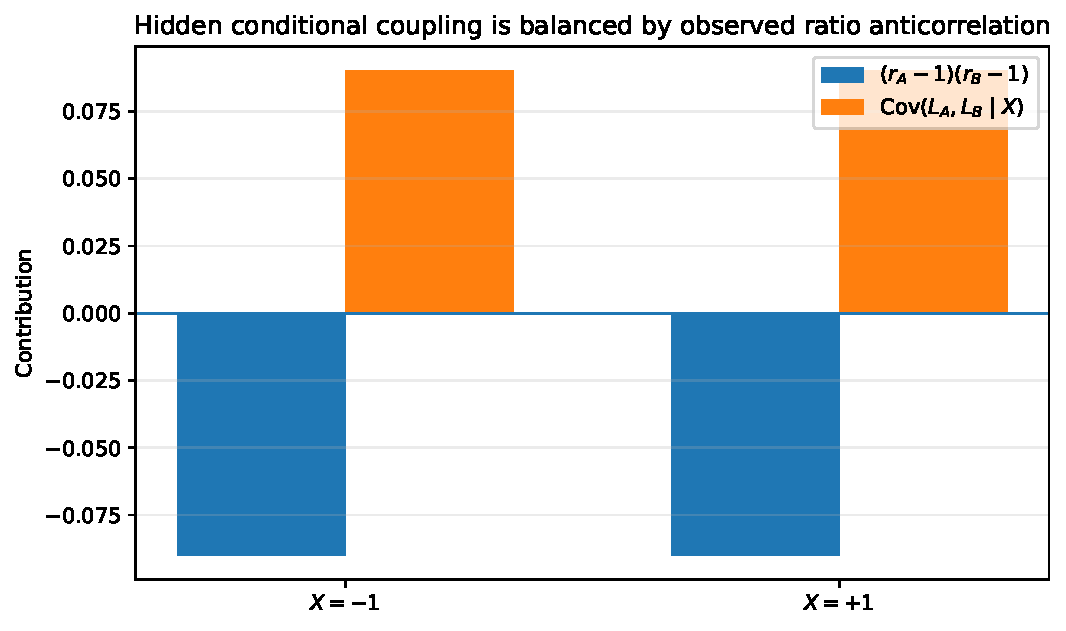
\includegraphics[width=0.82\linewidth]{figures/latent_conservation.pdf}
\caption{The latent conservation simulation.  Pointwise conditional covariance of the complete factors is balanced by anticorrelation of the observed primitive ratios.}
\label{fig:latent-conservation}
\end{figure}

These \(L_A,L_B\) are coordinated multi-source tilts.  They satisfy complete-state multiplicative flatness, which is all that the marginalization identity requires, but they are not single-mechanism ratios on a simple DAG over independent \((X,U)\).  An on-model parent-centered construction can replace them when locality itself is the object of simulation.

\subsection{Implementation inconsistency}

Let the primitive ratios be \(1+aX_1\) and \(1+bX_2\), but let the combined intervention acquire an additional normalized implementation factor
\begin{equation}
\frac{1+\gamma X_1X_2}{1+ab\gamma}.
\end{equation}
Then
\begin{equation}
\kappa(X_1,X_2)=
\log(1+\gamma X_1X_2)-\log(1+ab\gamma).
\end{equation}
With \(a=0.45\), \(b=0.35\), and \(\gamma=0.4\), curvature is \(-0.571921\) when \(X_1X_2=-1\) and \(0.275377\) when \(X_1X_2=1\).  Setting \(\gamma=0\) is an exact negative control.

\begin{figure}[t]
\centering
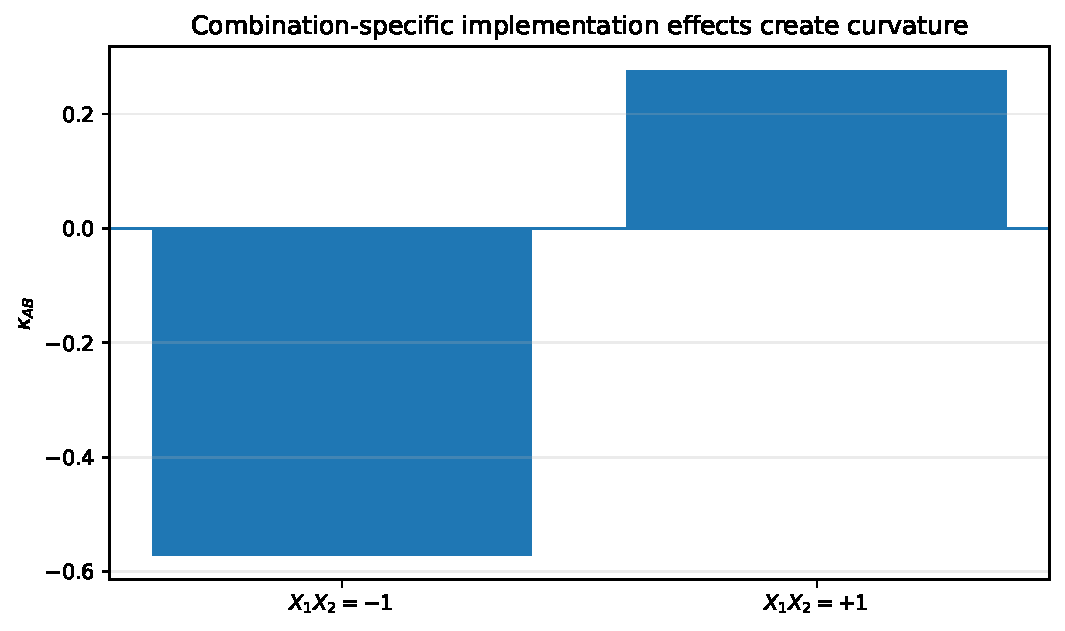
\includegraphics[width=0.82\linewidth]{figures/implementation_inconsistency.pdf}
\caption{Combination-specific implementation effects create curvature even when the nominal primitive perturbations are conceptually distinct.}
\label{fig:implementation}
\end{figure}

\section{Empirical programs}

\subsection{Engineered feature flags}

An engineered system offers the cleanest first validation because assignment, implementation, and telemetry can be controlled.  Select two or more flags believed to alter distinct modules.  Randomize them independently at the request, session, host, or deployment-unit level, and collect a rich state including local module outputs, queues, resource pressure, latency distributions, error traces, and intervention-delivery metadata.

The protocol is:
\begin{enumerate}
\item verify product assignment and no state-dependent inclusion;
\item define negative-control flag pairs with separate implementation paths;
\item localize each primitive regime node;
\item run simultaneous deletion-equivalence orientation;
\item run GCM/wGCM projections and a joint multinomial interaction diagnostic;
\item hold out selected combinations and predict their full state distributions from primitive ratios;
\item add candidate telemetry when curvature is found and apply the nested state-expansion test;
\item cluster uncertainty at the true randomization unit.
\end{enumerate}

This experiment can distinguish nonlinear product behavior from shared-resource coupling and from missing telemetry.  Resolution-V fractions become useful once the number of flags exceeds what a full factorial can support.

\subsection{Combinatorial Perturb-seq}

Combinatorial Perturb-seq provides single and paired genetic perturbations with rich single-cell phenotypes \citep{norman2019perturbseq}.  For each pair \((A,B)\), fit the four-corner model
\begin{equation}
\eta_{ab}(x)=af_A(x)+bf_B(x)+abf_{AB}(x).
\end{equation}
Estimate curvature at the biological-replicate level, not by treating cells as independent randomized units.  Separate intervention-delivery curvature using alternative guides, guide-position swaps, expression or knockdown measurements, and non-targeting controls.

The central analysis is two-dimensional.  Compare conventional genetic interaction summaries with full-distribution curvature.  The decisive cases are perturbation pairs with strong outcome epistasis but low curvature, and pairs with weak selected-outcome interaction but high distributional curvature.  Same-complex or same-pathway pairs may be enriched for curvature, but that is an empirical hypothesis, not a theorem.

Fit control and single perturbations, self-normalize the product ratio, and predict held-out paired distributions.  Compositional perturbation predictors such as CPA impose additive latent structure \citep{lotfollahi2023cpa}; mechanism interferometry specifies where exact additivity belongs---the log density of a design-sufficient state---and supplies a test for when the prior fails.

\section{Failure taxonomy and limitations}

A nonzero curvature field proves that the proposed regime family is not closed under the asserted composition law.  It does not uniquely identify the cause.  Important possibilities are:
\begin{enumerate}
\item genuine mechanism coupling;
\item two perturbations sharing a target;
\item omitted common state;
\item state-dependent selection;
\item combination-specific implementation or dosage;
\item regime-dependent measurement;
\item poor overlap or estimation error;
\item incorrect correspondence between nominal and actual interventions.
\end{enumerate}

Likewise, zero curvature is relative.  It does not prove that no latent variables exist; it says that the chosen perturbations do not expose a failure of closure at the observed resolution.

The strongest graph-identification conclusions require ratio faithfulness, deletion faithfulness, adequate target coverage, and acyclicity.  Conditional-independence testing remains difficult in high dimension \citep{shah2020gcm}.  Hard interventions may fall outside the common-support calculus.  In time series, whole-trajectory ratios can have variance that grows exponentially with horizon; estimation should occur at the transition level, pooling local conditional ratios with trajectory-level uncertainty.  Static DAGs do not directly cover feedback at equilibrium, where Modular Response Analysis provides an important complementary tradition \citep{bruggeman2002mra,kholodenko2002untangling}.

\section{Relation to prior work and novelty}

The locality result is the Markov blanket of a context node in an augmented causal graph, squarely connected to causal discovery from mechanism changes and Joint Causal Inference.  The density ratio is classical change of measure and has recently been promoted as a pointwise causal object \citep{mahadevan2026density}.  The exact pairwise product identity and four-corner null have direct precedent in \citet{xu2024pairwise}, including an empirical study using microscopy readouts from 50 gene-pair knockouts.  That work strengthens the case that distribution-level four-corner tests are empirically viable on unstructured biological data.

The certificate also admits an exact sparsity reading.  Under modularity, the master log-linear model \eqref{eq:master-loglinear} confines all \(2^K\) regime log laws, pointwise in \(x\), to the \((K+1)\)-dimensional main-effects subspace spanned by the baseline log density and one potential per primitive perturbation; without modularity the family occupies up to \(2^K\) unconstrained functions.  Every nonvanishing curvature field is an additional function that the regime family forces the description to carry, and the M\"obius expansion \eqref{eq:mobius-curvature} enumerates these correction terms order by order.  Relative to an already specified labeled cube, modularity is therefore a maximal-parsimony statement about the regime family, and curvature terms are its epicycles.  This is a bridge of principle to the algorithmic-independence-of-mechanisms and minimum-description-length traditions in causal inference \citep{janzing2010algorithmic,grunwald2007mdl}, not a codelength theorem: the object constrained here is the exact dimension of a function-valued design subspace, derived from an explicit interventional algebra rather than postulated about observational complexity.  The practical corollary is a tie-breaking principle used throughout the protocol: among localized supports and representations that meet the same held-out sufficiency threshold, prefer the most parsimonious one, because by locality the true support \(\{t\}\cup\pa(t)\) is, under ratio and deletion faithfulness and adequate data, the smallest support consistent with the regime information.

This compression reading is a restricted proposal principle, not a definition
of causal coordinates.  Real environments can be fat interventions, and
componentwise invertible or other structure-preserving reparameterizations can
retain sparse changes.  Change sparsity alone therefore ranks candidate
factorizations; it does not identify one.  The certificate conditions test
different consequences of a proposed sparse-mechanism account: locality
restricts a primitive ratio to one causal family, conditional normalization
asks whether it can be a valid replacement at a proposed target, square
flatness tests context-invariant composition of proposed distinct
replacements, and the conservation identities relate complete- and
observed-state curvature only after a complete flat factorization has been
separately assumed.  Deletion equivalence orients only a credible single-target
family under deletion faithfulness.  None of these conditions by itself
measures causal sparsity or identifies a hidden coordinate.

The differential-geometric program of \citet{mahadevan2026infinitesimal} is conceptually adjacent: failures of intervention-induced fields to close can witness unmodeled structure.  Its Lie brackets measure sequential infinitesimal noncommutativity, while the present construction is a finite symmetric mixed difference on a Boolean design and requires no smooth intervention path.

No individual probability identity in this paper should be claimed as novel.  Relative to the complete-cube, common-support, proposed-DAG, and distinct-target assumptions of \cref{thm:certificate}, the narrow contribution is the assembled object:
\begin{equation}
\boxed{
\text{local family support}
+
\text{targetwise normalization}
+
\text{gauge-invariant square flatness}
}
\end{equation}
\begin{equation}
\boxed{
\Longleftrightarrow
\text{existence of a context-invariant modular soft-intervention model},
}
\end{equation}
together with ratio-free orientation, support-error diagnostics, exact latent conservation, missing-information interpretation, state-expansion conservation, and the dual inference architecture.  This is a literature-based novelty assessment, not proof of priority.

\section{Conclusion}

Mechanism interferometry treats a factorial family of empirical regimes as one constrained mathematical object.  The first implication below assumes ratio and minimal-support faithfulness; the second assumes credible single-target semantics and deletion faithfulness; and the fourth assumes the regular dominated smooth family and zero complete-state cross-Hessian used in the missing-information derivation.  With those premises retained, the central logic can be summarized in four lines:
\begin{align}
\text{locality}
&\Longrightarrow
\text{which causal family changed},\\
\text{deletion invariance}
&\Longrightarrow
\text{which family member is the target},\\
\text{nonzero square curvature}
&\Longrightarrow
\text{where autonomous composition fails},\\
\text{conditional score covariance}
&\Longrightarrow
\text{how much joint mechanism information was lost}.
\end{align}

The method separates outcome-scale nonlinearity from failure of closure at the chosen state representation.  Curvature alone cannot then distinguish genuine mechanism coupling from representational incompleteness: the same observed regime laws can admit either explanation.  State expansion, intervention metadata, and implementation controls supply discriminative follow-up evidence, but do not turn that observational ambiguity into an algebraic identification result.  Evidence for causality no longer rests on one significant coefficient.  It rests on simultaneous satisfaction of locality, normalization, square closure, moment restrictions, held-out compositional prediction, overlap requirements, and implementation negative controls.  The resulting overdetermination is the source of evidential strength.

Across many environments, this algebra suggests a guarded path toward causal mechanism tomography.  Discovery splits can search for recurring log-law transports, parsimonious stable supports, response sets, candidate assignment discontinuities, and externally recorded actions.  Conditional normalization can then distinguish local mechanism candidates from arbitrary low-rank factors, while independently observed squares and held-out combinations test whether the proposed vocabulary actually composes.  Oriented local families and response propagation may assemble a partial causal order; a randomized, discontinuity, instrumental-variable, or temporal contract may instead identify one query-specific effect without identifying a global graph.  All such searches remain proposal mechanisms until their candidate library, unit split, selection assumptions, and strategy-specific premises are frozen and tested on independent data.  Thus the scalable objective is not to force a DAG from a large table, but to discover the strongest causal question the available environment family can support, expose the premise that rows cannot establish, and recommend the cheapest new measurement or perturbation that separates the surviving explanations.

\appendix

\section{Additional proofs}
\label{app:proofs}

\subsection{Square flatness implies all-order flatness}

Fix \(x\) and suppress it.  Let \(h:\{0,1\}^K\to\R\).  For coordinate \(j\), define \(\delta_j(s)=h(s+e_j)-h(s)\) wherever \(s_j=0\).  If every square contrast vanishes, then for every \(k\ne j\),
\begin{equation}
\delta_j(s+e_k)-\delta_j(s)=\Delta_k\Delta_jh(s)=0.
\end{equation}
Every two vertices of the subcube \(s_j=0\) are connected by flips of coordinates other than \(j\).  Hence \(\delta_j(s)=\delta_j(0)\).  Summing along a monotone path from \(0\) to \(s\) gives
\begin{equation}
h(s)=h(0)+\sum_js_j\delta_j(0).
\end{equation}
Every mixed difference of order at least two annihilates this affine form.

\subsection{Peeling reconstruction from unlabeled families}

Let \(\calF=\{F_i:i\in[d]\}\) with \(F_i=\{i\}\cup\pa(i)\).  Maintain identified set \(U\).  If \(U\ne[d]\), choose the earliest node \(i\notin U\) in a topological ordering restricted to unidentified nodes.  Every parent of \(i\) lies in \(U\), so
\begin{equation}
F_i\setminus U=\{i\}.
\end{equation}
Conversely, if an unassigned family reduces to \(\{i\}\), its target must be \(i\), because every family contains its own target and no other unidentified element.  Assign the family, recover \(\pa(i)=F_i\setminus\{i\}\), add \(i\) to \(U\), and iterate.  This proves uniqueness.

\subsection{Preservation under design sufficiency}

For any two corners \(s,t\), Bayes' rule under pooling law \(\rho\) gives
\begin{equation}
\log\frac{p_s(o)}{p_t(o)}
=
\log\frac{P_\rho(S=s\mid O=o)}{P_\rho(S=t\mid O=o)}
-
\log\frac{\rho_s}{\rho_t}.
\end{equation}
If \(S\perp O\mid Z\), the posterior odds depend on \(o\) only through \(z=\phi(o)\).  Every linear contrast of regime log ratios, including all M\"obius curvatures, is therefore preserved.

\subsection{Nested state expansion}

By the conditional law of total covariance,
\begin{align}
\Cov(L_A,L_B\mid X)
={}&
\E[\Cov(L_A,L_B\mid X,W)\mid X]\\
&+
\Cov(\E[L_A\mid X,W],\E[L_B\mid X,W]\mid X).
\end{align}
Substitute
\begin{equation}
\Cov(L_A,L_B\mid X)=r_A^Xr_B^X(e^{\kappa_X}-1)
\end{equation}
and the analogous identity at \((X,W)\).

\section{Partial-design estimability}
\label{app:partial-designs}

Let \(D=\{s^{(1)},\ldots,s^{(n_D)}\}\).  Define the main-effects matrix
\begin{equation}
M_D=
\begin{bmatrix}
1&s_1^{(1)}&\cdots&s_K^{(1)}\\
\vdots&\vdots&&\vdots\\
1&s_1^{(n_D)}&\cdots&s_K^{(n_D)}
\end{bmatrix}.
\end{equation}
For a categorical product grid, replace the \(K\) binary columns by one
indicator for each nonbaseline level of each family.  The coded column count is
\begin{equation}
q=1+\sum_j(|\mathcal A_j|-1).
\end{equation}
At each \(x\), the flat model is \(h_D(x)=M_D\beta(x)\).  A contrast \(c^\top h_D(x)\) is a testable implication of flatness exactly when \(c\in\ker(M_D^\top)\).  The dimension of the lack-of-fit space is
\begin{equation}
n_D-\operatorname{rank}(M_D).
\end{equation}
The additive coefficient functions are unique exactly when
\(\operatorname{rank}(M_D)=q\); otherwise every feasible algebraic solution
lies in an affine functional fiber directed by \(\ker(M_D)\).  A linear
functional of the potentials is algebraically identified exactly when its
coefficient vector lies in the row space of \(M_D\).  These are design-space
facts only.  Locality and exponential conditional normalization define the
nonlinear causal-completion fiber in
\eqref{eq:causal-completion-fiber} and can rule out a linearly saturated design
or restore uniqueness in a rank-deficient one.
An implementation should compute a numerically stable basis of this null space, map familiar face contrasts into it, and report which directions are untested or aliased.  For binary fractions, standard defining relations and generalized word-length patterns can be carried over pointwise.

The six-corner design \(\{0,1\}^3\setminus\{000,111\}\) has \(n_D=6\) and rank four.  It has two independent lack-of-fit contrasts despite containing no complete square face.  This demonstrates why ``test all observed squares'' is complete only under a design-topology condition.

\section{Simulation derivations}

\subsection{Gaussian ratio identity}

For \(\phi_\sigma(z)=(2\pi\sigma^2)^{-1/2}\exp(-z^2/(2\sigma^2))\),
\begin{equation}
\frac{\phi_\sigma(y-1)}{\phi_\sigma(y+1)}
=
\exp\left(\frac{2y}{\sigma^2}\right).
\end{equation}
Writing \(R=e^{2y/\sigma^2}\),
\begin{equation}
\frac{\phi_\sigma(y-1)-\phi_\sigma(y+1)}
{\phi_\sigma(y-1)+\phi_\sigma(y+1)}
=
\frac{R-1}{R+1}
=
\tanh(y/\sigma^2).
\end{equation}

\subsection{Parity arithmetic}

Under either mechanism, \(P\) is uniform.  For each value of \(T\), summing over \(P\) gives probability \(1/2\), regardless of \(\eps\).  Hence both one-dimensional marginals are invariant, even though the conditional relation between \(P\) and \(T\) reverses.

\subsection{Implementation factor normalization}

Under primitive tilts, \(\E_{AB}^{\mathrm{flat}}[X_1X_2]=ab\).  Therefore
\begin{equation}
\E_{AB}^{\mathrm{flat}}[1+\gamma X_1X_2]=1+ab\gamma,
\end{equation}
which proves that the factor used in the implementation-inconsistency simulation is normalized.

\section{Longitudinal extension}

For a transition model,
\begin{equation}
p_e(x_{0:T})=p_e(x_0)\prod_{t=1}^Tp_e(x_t\mid x_{<t}).
\end{equation}
If only one transition mechanism changes, the log trajectory ratio is a sum of local transition log ratios.  Direct products can have exponentially growing second moments.  The implementation should therefore estimate transition-level ratios, pool across comparable transitions, and use trajectory- or subject-level resampling.  Feedback is represented by the unrolled temporal graph rather than by pretending that a static DAG contains no cycles.

\section{Software audit contract}

Every empirical run should emit a machine-readable audit bundle containing:
\begin{enumerate}
\item input fingerprints and schema version;
\item regime definitions, pooling proportions, and product-sampling check;
\item cross-fitting fold assignments and deterministic random seeds;
\item selection and overlap diagnostics;
\item localization stability paths;
\item simultaneous deletion-equivalence intervals and pass status;
\item exploratory proposal artifacts, their candidate-library fingerprints, tie rules, and recommendation-or-abstention status;
\item moment battery, GCM/wGCM projections with their serialized product-design evidence, and joint-model diagnostics;
\item estimator-family agreement results across the declared lens battery;
\item raw and self-normalized compositional predictions;
\item state-expansion comparisons;
\item negative-control results;
\item all warnings, abstentions, and strict-mode failures.
\end{enumerate}
The companion repository defines JSON schemas for these artifacts and a Rust workspace architecture for producing them.

This list is a contract for the mature system, not a claim that every item is
already production-ready.  The current implementation ships the exact
population algebra, categorical and partial-design geometry, manifest and
sampling audits, typed authority gates, deterministic proposal artifacts,
simulations, and a cluster-weighted discrete reference diagnostic.  It does
not yet ship the production cross-fitted joint regime model, a calibrated
global full-law closure test for flexible learners, nonparametric localization,
mechanism-dictionary identification from unknown environment codes, or the
Python/Arrow interfaces needed for million-row scientific tables.  The
autonomous survey is therefore proposal-only, and the reference histogram path
cannot issue a passed certificate.  These boundaries make the software's
current proof state inspectable instead of allowing the architecture to be
mistaken for completed statistical capability.

\subsection{Typed refusals}

The contract above is only enforceable if a refusal is a value rather than a
sentence in a log. The implementation therefore fixes a closed vocabulary of
blocking reason codes, and every gate in this paper emits one of them:

\begin{itemize}[nosep, leftmargin=1.5em, font=\ttfamily]
  \item non\_product\_sampling\_for\_gcm
  \item state\_dependent\_selection
  \item selection\_model\_unvalidated
  \item overlap\_failure
  \item orientation\_unresolved
  \item design\_contrast\_aliased
  \item no\_testable\_flatness
  \item non\_square\_contrasts\_required
  \item negative\_control\_curvature
  \item estimator\_family\_disagreement
  \item cluster\_spans\_regimes
  \item missing\_regime\_data
  \item empty\_common\_support
  \item declared\_empirical\_quota\_mismatch
  \item duplicate\_provenance
\end{itemize}

Informational findings carry a separate declared set, currently
\texttt{estimator\_family\_agreement} and
\texttt{histogram\_not\_a\_certificate}.  The split is deliberate rather than
bookkeeping.  An informational code records what a run established, never a
licence to proceed, and the first of these is the clearest case: agreement
across the estimator lens battery is diagnostic and certifies nothing on its
own, so a consumer that treated it as a gate would invert the very asymmetry
the battery is built on.  Both sets are declared in one place, so the
vocabulary is discoverable by a downstream reader rather than recoverable only
by reading every emission site.

The last of these enforces an append-only evidence ledger: binding a provenance
key twice with different values preserves the first write and records the
rejected one, so a later stochastic stage cannot silently overwrite an earlier
seed, randomization unit, or source fingerprint. Each preflight report also
carries the canonical hash of the manifest it validated, which binds a verdict
to the exact input that produced it.

A run terminates in one of four certificate states, \emph{passed},
\emph{failed}, \emph{abstained}, or \emph{diagnostic\_only}, and the
distinction between the last three is the substance rather than the packaging.
\emph{Failed} asserts that a certificate condition was tested and rejected;
\emph{abstained} asserts that the run declined to answer; and
\emph{diagnostic\_only} marks a result that may inform but can never be
promoted. A projection that tests no certificate condition therefore cannot
report \emph{failed}, because it has nothing to reject: the shipped
cluster-weighted histogram implementation of the four-law functionals returns
\emph{abstained} on every clean run by construction. It is a diagnostic that
can never certify, and saying so in the type is what prevents an eventual
reader from treating a quiet run as a passing one.

\subsection{Typed certificate gates}

A single boolean verdict cannot say which condition failed, so the four
certificate conditions are carried as typed values rather than collapsed into
one flag. Locality, conditional normalization, square flatness, and orientation
are each recorded as \emph{established}, \emph{refuted}, or \emph{unresolved},
and the terminal state is derived from that record rather than supplied
alongside it. The distinction is not cosmetic. ``The certificate failed'' and
``square flatness was rejected while orientation was never resolved'' license
entirely different next experiments, and only the second tells an experimenter
where to spend the next randomization. Carrying the gates also makes the
derivation auditable after the fact: a report states the inputs from which its
status follows, so a reader can recompute the verdict rather than trust it.

\subsection{Dependencies are load-bearing assumptions}

An audit system inherits the correctness of everything it reads with. The
tabular adapter therefore audits its own backend: every cell returned by the
sibling dataframe reader is compared against the reference tokenizer, and any
disagreement is a refusal naming the row, the column, and both values.

This is not hypothetical rigour. The reviewed revision of that reader rendered
the identifiers \texttt{007} and \texttt{7} as the same string, which merges two
distinct assignment units and pools their observations into a single
randomization unit, and it flattened the design label \texttt{00} to
\texttt{0}, erasing the distinction between two regimes. Neither failure raises
an error. Both produce a fluent report about a different experiment than the
one that was run, and the corrupted quantity is exactly the one on which the
spanning-cluster refusal is conditioned, so the failure can both manufacture
and mask the audit that would have caught it.

Version pinning does not detect this class of fault, because a pin records
which code ran and not whether it preserved the data. The comparison costs one
pass over the cells and converts an unverified assumption about a dependency
into either a checked fact or a typed refusal, which is the same standard the
rest of the protocol applies to assumptions about the world.

\subsection{Authority tiers under incomplete contracts}

Three of the four contracts a certificate requires admit partial data-driven
resolution: regimes can be discovered from context columns, sampling
proportions estimated from corner counts, and randomization units guessed
conservatively and audited at the coarsest plausible clustering. The fourth
does not. State-independent selection within regime cannot be established from
observed rows at all, because two models with different underlying laws and
different inclusion mechanisms can induce identical selected data. Any
procedure claiming to establish it from rows alone is producing a false
positive rather than a discovery.

Outputs are therefore graded rather than merely flagged. Tier~A is certified
and requires the declared sampling, selection, and clustering contracts.
Tier~B is a corroborated diagnostic: every internally checkable audit passed,
serialized as \emph{diagnostic\_only} together with a typed checklist, with no
scalar score and no total ordering, so a reader always sees which gates passed
and which were inapplicable. Tier~C is a proposal, quarantined under the
proposal-adapter boundary. Tier~B is the operating point
this architecture adds: stronger than a discovery algorithm's edge weight,
deliberately weaker than a certificate, and unable to overclaim because
overclaiming is a type error rather than a matter of restraint.

\subsection{The report leads with what it refused}

The audit emits a human-readable report whose ordering is fixed by the
implementation rather than chosen per run. The first heading is the certificate
status; the second section is the abstentions, each with its reason code; the
informational findings come last. A report cannot open with a table of
significance statistics, and a test asserts as much, because the ordering of a
document is itself a claim about what matters in it. The conventional
arrangement, in which the estimates lead and the caveats trail, is well suited
to a reader looking for a result and poorly suited to one who needs to know
whether the result is admissible.

\subsection{Proposal-side discovery and its quarantine}

Two proposal-layer artifacts extend the boundary to the many-environment
setting without weakening it. A scout freezes candidate shift structure
discovered across environments, and a shift-factorization proposal records a
candidate decomposition of observed shifts into reusable factors. Both are
frozen with complete adapter provenance, both serialize with authority
\texttt{proposal\_only}, and neither depends on the audit or design verdict
types, so a frozen artifact can order later work but cannot be converted into a
certificate gate, target, edge, or invariant. The type system, not the
analyst's restraint, is what prevents a discovery from being read as a finding.

A dataset gauntlet complements them on the intake side. Rather than asking
whether a dataset is interesting, it asks which of the certificate's contracts
that dataset could possibly satisfy, and records the answer before any
estimation is attempted. Most candidate datasets fail at the selection contract,
and discovering that in advance is cheaper than discovering it in a verdict that
has to be withdrawn.

\printbibliography

\end{document}
